\documentclass[conference]{IEEEtran}
\IEEEoverridecommandlockouts
\usepackage{cite}
\usepackage{amsmath,amssymb,amsfonts}
\usepackage{algorithm}
\usepackage{algpseudocode}
\usepackage{graphicx}
\usepackage{textcomp}
\usepackage{xcolor}
\usepackage{booktabs}
\usepackage{multirow}
\usepackage{array}
\usepackage{url}
\usepackage[hidelinks]{hyperref}
\usepackage{microtype}
\def\BibTeX{{\rm B\kern-.05em{\sc i\kern-.025em b}\kern-.08em T\kern-.1667em\lower.7ex\hbox{E}\kern-.125em X}}
\graphicspath{{figures/}}
\newcommand{\NTrain}{602}
\newcommand{\NVal}{206}
\newcommand{\NTest}{206}
\newcommand{\TBestEpoch}{2}
\newcommand{\TTrainHours}{3.6}
\newcommand{\TMaxTok}{580}
\newcommand{\TMeanTok}{301}
\newcommand{\TTrunc}{0}
\newcommand{\DBestEpoch}{1}
\newcommand{\DTrainHours}{2.3}
\newcommand{\DMaxTok}{580}
\newcommand{\DMeanTok}{301}
\newcommand{\DTrunc}{0}
\newcommand{\TestAcc}{0.626}
\newcommand{\TestMF}{0.333}
\newcommand{\TestEvF}{0.123}
\newcommand{\BaseAcc}{0.437}
\newcommand{\BaseMF}{0.234}
\newcommand{\BaseEvF}{0.000}
\newcommand{\BaseInvalid}{0}
\newcommand{\TestInvalid}{0}
\newcommand{\MajAcc}{0.626}
\newcommand{\MajMF}{0.272}
\newcommand{\NGoldEmpty}{145}
\newcommand{\NGoldNon}{61}
\newcommand{\EmptyOK}{0.959}
\newcommand{\EmptyFalseCit}{6}
\newcommand{\NContradict}{131}
\newcommand{\NLabelErr}{77}
\newcommand{\TestAccLo}{0.472}
\newcommand{\TestAccHi}{0.748}
\newcommand{\TestMFLo}{0.237}
\newcommand{\TestMFHi}{0.408}
\newcommand{\TestEvFLo}{0.024}
\newcommand{\TestEvFHi}{0.259}
\newcommand{\BaseAccLo}{0.367}
\newcommand{\BaseAccHi}{0.539}
\newcommand{\BaseMFLo}{0.190}
\newcommand{\BaseMFHi}{0.273}
\newcommand{\BaseEvFLo}{0.000}
\newcommand{\BaseEvFHi}{0.000}

\newcommand{\GNTrain}{602}
\newcommand{\GNVal}{206}
\newcommand{\GNTest}{206}
\newcommand{\GTBestEpoch}{2}
\newcommand{\GTTrainHours}{0.3}
\newcommand{\GTMaxTok}{580}
\newcommand{\GTMeanTok}{301}
\newcommand{\GTTrunc}{0}
\newcommand{\GDBestEpoch}{2}
\newcommand{\GDTrainHours}{0.1}
\newcommand{\GDMaxTok}{580}
\newcommand{\GDMeanTok}{301}
\newcommand{\GDTrunc}{0}
\newcommand{\GTestAcc}{0.709}
\newcommand{\GTestMF}{0.460}
\newcommand{\GTestEvF}{0.384}
\newcommand{\GBaseAcc}{0.146}
\newcommand{\GBaseMF}{0.111}
\newcommand{\GBaseEvF}{0.151}
\newcommand{\GBaseInvalid}{1}
\newcommand{\GTestInvalid}{0}
\newcommand{\GMajAcc}{0.626}
\newcommand{\GMajMF}{0.272}
\newcommand{\GNGoldEmpty}{145}
\newcommand{\GNGoldNon}{61}
\newcommand{\GEmptyOK}{0.959}
\newcommand{\GEmptyFalseCit}{10}
\newcommand{\GKVAllMatch}{27/27}
\newcommand{\GKVSpeedup}{18.7}
\newcommand{\GKVBigIn}{512}
\newcommand{\GKVBigOut}{128}
\newcommand{\GAttnWorstErr}{1.4e-06}
\newcommand{\GSpecBestSpeedup}{0.81}
\newcommand{\GSpecBestK}{6}
\newcommand{\GSpecBestDraft}{finetuned draft}
\newcommand{\GSpecHF}{6/6 prompts: HF assisted == ours == cached greedy}
\newcommand{\GNContradict}{130}
\newcommand{\GNLabelErr}{60}
\newcommand{\GTestAccLo}{0.578}
\newcommand{\GTestAccHi}{0.818}
\newcommand{\GTestMFLo}{0.359}
\newcommand{\GTestMFHi}{0.554}
\newcommand{\GTestEvFLo}{0.276}
\newcommand{\GTestEvFHi}{0.476}
\newcommand{\GBaseAccLo}{0.104}
\newcommand{\GBaseAccHi}{0.198}
\newcommand{\GBaseMFLo}{0.087}
\newcommand{\GBaseMFHi}{0.134}
\newcommand{\GBaseEvFLo}{0.083}
\newcommand{\GBaseEvFHi}{0.226}


\begin{document}

\title{Criterion-Level Clinical-Trial Eligibility Screening with a Fine-Tuned Small Transformer:\\
KV-Cached Decoding, Tiled Online-Softmax Attention and Speculative Decoding on Commodity CPUs}

\author{\IEEEauthorblockN{[AUTHOR NAME]}
\IEEEauthorblockA{[Roll No.] \\ Department of [Department], [University]\\
Generative AI (Semester 7), Assignment 2\\
[email address]}}

\maketitle

\begin{abstract}
Matching a patient to a clinical trial requires deciding, for every inclusion and exclusion criterion, whether the patient record satisfies it, contradicts it, or simply does not say. We build and evaluate a complete, locally executable system for this criterion-level task on the TrialGPT Criterion Annotations corpus using a patient-grouped 37/8/8 split. An open-weight decoder (SmolLM2-1.7B-Instruct on a free GPU; a 360M variant on a laptop CPU) is adapted with LoRA to emit a structured JSON answer containing one of the dataset's expert label categories and the IDs of the supporting patient sentences. On the untouched test split the adapted 1.7B model reaches \GTestAcc{} accuracy and \GTestMF{} macro-F1 (zero-shot base model: \GBaseAcc{} and \GBaseMF{}; majority-label baseline: \GMajAcc{} and \GMajMF{}), with micro evidence-sentence F1 of \GTestEvF{}. An error analysis shows that the gain comes from inclusion criteria, whereas for exclusion criteria the model collapses to the majority label \emph{not excluded}. Beyond accuracy, we re-implement the inference stack from first principles: a Llama-style decoder with an explicit, rollback-capable KV cache; a tiled attention kernel with online softmax; and greedy speculative decoding with a LoRA-adapted draft model. Every mechanism is validated for exact agreement with a reference path (the cache is \GKVSpeedup$\times$ faster than recomputation at 512+128 tokens; speculative decoding is exact but, honestly, slower than greedy with the chosen draft) and benchmarked for latency, throughput and memory on both a GPU and a laptop CPU. The pieces are integrated in a browser application that exposes per-criterion evidence, a live decoding-mode comparison and exportable reports. The system is an educational prototype and not a clinical decision tool.
\end{abstract}

\begin{IEEEkeywords}
clinical trial matching, eligibility criteria, LoRA, KV cache, online softmax, speculative decoding, small language models
\end{IEEEkeywords}

\section{Introduction}
Enrolling the right patients in a clinical trial is slow largely because eligibility is written as free text. A trial protocol lists a dozen or more inclusion and exclusion criteria; a clinician must read each one against the patient's record. Large language models (LLMs) can perform this reading, and TrialGPT~\cite{jin2024trialgpt} showed that a GPT-4-based pipeline can predict criterion-level eligibility and cite the supporting note sentences with accuracy approaching that of human experts. That work, however, relies on a proprietary model behind a paid API, which is unsuitable for privacy-sensitive records and for students without budget.

\textbf{Problem statement.} Given (i) a patient description whose sentences are numbered, (ii) a criterion type (inclusion or exclusion), and (iii) the criterion text, predict the expert eligibility label---including \emph{not enough information} and \emph{not applicable}, which are never collapsed into yes/no---and the IDs of the sentences that justify it. We require the solution to run on freely available hardware with an open-weight model, to be evaluated on a fixed, patient-grouped held-out split, and to expose the Transformer inference machinery explicitly rather than through a library switch.

\textbf{Contributions.}
\begin{enumerate}
\item A reproducible supervised adaptation of a 360M-parameter decoder (and a 135M draft) on the prescribed corpus, with before/after comparison on identical validation and test cases, plus per-class, per-criterion-type and evidence-level metrics and an error analysis.
\item A from-scratch Llama-architecture decoder with an explicit KV cache (growth, rollback, position handling), verified against the Hugging Face implementation.
\item A tiled attention routine using the online-softmax recurrence, validated against a reference attention across shapes, masks and cache offsets.
\item A greedy speculative decoder with synchronised target/draft caches whose outputs are token-identical to greedy target decoding, with acceptance statistics and an honest speed analysis.
\item A browser application that ties these parts together and lets a user compare decoding modes live.
\end{enumerate}

The remainder of the paper is organised as follows. Section~II reviews related work, Section~III describes data, model and algorithms, Section~IV the experimental setup, Section~V the results, and Section~VI limitations and conclusions.

\section{Related Work}
\textbf{Clinical-trial matching.} The patient descriptions in our corpus originate from the SIGIR 2016 test collection of Koopman and Zuccon~\cite{koopman2016sigir}, which pairs short synthetic patient summaries with trials judged for relevance. TrialGPT~\cite{jin2024trialgpt} decomposes matching into retrieval, criterion-level prediction with evidence, and ranking, and released the expert criterion-level annotations~\cite{ncbi2024dataset} that serve as the benchmark here (1\,015 annotated patient--criterion pairs over 53 patients in the public file). We use only the criterion-level task and replace GPT-4 with a small local model; the GPT-4 outputs distributed with the dataset are discarded.

\textbf{Parameter-efficient adaptation.} LoRA~\cite{hu2022lora} freezes the pre-trained weight $W$ and learns a low-rank update $\Delta W=\tfrac{\alpha}{r}BA$, so optimizer state is kept only for the small matrices $A,B$. QLoRA~\cite{dettmers2023qlora} additionally stores the frozen base in 4 bits, which saves memory on GPUs but depends on CUDA kernels that are unavailable to us; at 360M parameters fp32 weights occupy only about 1.4\,GB, so we use plain LoRA.

\textbf{Small open decoders.} SmolLM2~\cite{allal2025smollm2} provides 135M, 360M and 1.7B Llama-style~\cite{touvron2023llama} models with RMSNorm~\cite{zhang2019rmsnorm}, SwiGLU~\cite{shazeer2020glu}, rotary embeddings~\cite{su2024roformer} and grouped-query attention~\cite{ainslie2023gqa}, all sharing one tokenizer---a prerequisite for speculative decoding. Qwen2.5-0.5B~\cite{qwen2024qwen25} is a comparable alternative with a much larger vocabulary and no smaller sibling.

\textbf{Efficient attention.} Standard attention~\cite{vaswani2017attention} materialises a $T\times T$ score matrix. The online normaliser~\cite{milakov2018online} computes softmax in one pass with a running maximum and sum; combined with tiling this yields memory-efficient exact attention~\cite{rabe2021selfattention} and its IO-aware GPU realisation FlashAttention~\cite{dao2022flashattention}. We implement the recurrence in PyTorch for correctness and analysis, not for speed.

\textbf{KV caching and speculative decoding.} Autoregressive generation recomputes nothing if past keys and values are cached; managing that cache is a central serving problem~\cite{pope2023efficiently,kwon2023pagedattention}, and multi-query/grouped-query attention shrinks it~\cite{shazeer2019mqa,ainslie2023gqa}. Speculative decoding~\cite{leviathan2023speculative,chen2023speculative} lets a cheap draft model propose several tokens that the target verifies in one forward pass; with greedy decoding the output equals the target's own greedy output, and the speed-up depends on the acceptance rate and the draft/target cost ratio.

\section{Materials and Methods}

\subsection{Dataset, Split and Leakage Control}
We use only the TrialGPT Criterion Annotations file (1\,015 rows, 53 patients)~\cite{ncbi2024dataset}. Each row holds a patient note whose sentences are numbered (\texttt{0. \ldots}), a trial identifier and title, the criterion type and text, the expert label, and the expert evidence sentence IDs. The file also contains GPT-4 explanations, sentence IDs, labels and a correctness flag; these four columns are dropped at load time (\texttt{LEAKY\_COLUMNS} in \texttt{src/data.py}) so they cannot reach a prompt or a metric. The upstream \texttt{training} flag is ignored.

The split follows the assignment protocol: the 53 unique patient IDs are sorted, shuffled in place with \texttt{numpy.random.default\_rng(42)}, and the first 37, next 8 and last 8 IDs form train, validation and test. A programmatic check asserts that the three ID sets are disjoint, jointly cover all patients and account for every annotation; the manifest is saved as \texttt{data/processed/split\_manifest.json}. Table~\ref{tab:split} gives the resulting sizes. One annotation (ID 883) has no criterion text in the source file, so there is nothing to predict; it stays in the manifest counts but is excluded from training and evaluation, leaving \NTrain/\NVal/\NTest{} usable rows. Table~\ref{tab:labels} shows the label distribution: the classes \emph{excluded} and \emph{not included} are rare, and the test split contains no \emph{excluded} example at all, which affects how macro-F1 must be read.

\begin{table}[t]\centering\caption{Patient-grouped split (seed 42).}\label{tab:split}
\small\begin{tabular}{lrrrr}\toprule
Split & Patients & Annotations & Incl. & Excl. \\\midrule
train & 37 & 602 & 215 & 387 \\
validation & 8 & 206 & 66 & 140 \\
test & 8 & 206 & 75 & 131 \\
\bottomrule\end{tabular}
\end{table}
\begin{table}[t]\centering\caption{Expert label distribution per split (usable rows).}\label{tab:labels}
\small\begin{tabular}{lrrr}\toprule
Label & Train & Val. & Test \\\midrule
included & 88 & 35 & 27 \\
not included & 13 & 3 & 7 \\
excluded & 8 & 2 & 0 \\
not excluded & 291 & 101 & 91 \\
not enough info. & 174 & 53 & 66 \\
not applicable & 28 & 12 & 15 \\
\bottomrule\end{tabular}
\end{table}

\subsection{Task Formulation, Prompt and Output Schema}
The input is rendered through the model's ChatML template with a fixed system message, the numbered note, the criterion type, the criterion text and the list of labels allowed for that type (four per type: \emph{included/not included} or \emph{excluded/not excluded}, plus \emph{not enough information} and \emph{not applicable}). The target is a compact JSON object,
\begin{center}\small\texttt{\{"label": "not excluded", "evidence": [3, 5]\}}\end{center}
followed by the end-of-turn token. Evidence IDs are the original sentence IDs of the note, sorted ascending; an empty list is a legitimate answer. The parser accepts the JSON form, falls back to a lenient search for a label string, and marks anything else \emph{invalid}, which always counts as an error. Notes are short (mean prompt+answer length \TMeanTok{} tokens, maximum \TMaxTok{} with the SmolLM2 tokenizer), so with a 1\,024-token limit \textbf{no example is truncated} (\TTrunc{} truncations); the code nevertheless counts truncation events and would report them.

\subsection{Model Candidates and Selection}
We study two hardware tiers with the same model family. Table~\ref{tab:cand} lists the candidates with properties computed directly from each model's published \texttt{config.json}: parameter count, fp32 weight memory (parameters $\times$ 4 bytes), layers, query/key-value heads, vocabulary, context window, the fp32 KV-cache cost per token ($2\cdot L\cdot H_{kv}\cdot d_{head}\cdot 4$ bytes), and the role each model plays in this work. All four are Apache-2.0 licensed decoders (Llama-style for SmolLM2, Qwen2-style for Qwen2.5-0.5B). The figures are derived, not benchmarked; the training and inference times that actually decided the configuration are reported in Section~\ref{sec:results}.

\textbf{Configuration~A (GPU, headline).} Target \textbf{SmolLM2-1.7B-Instruct}: 1.71\,B parameters, 24 layers, hidden size 2\,048, 32 query heads with 32 key/value heads (multi-head attention, 64-dimensional heads), SwiGLU feed-forward of width 8\,192, rotary embeddings ($\theta=1.3\times10^5$), 8\,192-token context, tied embeddings, 49\,152-token vocabulary; about 6.85\,GB in fp32. It trains on a free 15\,GB T4 with LoRA and fp16 autocast. Draft \textbf{SmolLM2-360M-Instruct} (same tokenizer). Larger options (e.g.\ 7--8B models) would require 4-bit quantisation and CUDA-only libraries and were not considered.

\textbf{Configuration~B (CPU).} Target \textbf{SmolLM2-360M-Instruct}: 32 layers, hidden size 960, 15 query heads sharing 5 key/value heads (grouped-query attention), feed-forward width 2\,560, 8\,192-token context; about 1.45\,GB in fp32 and trainable in hours on four CPU cores. Draft \textbf{SmolLM2-135M-Instruct} (30 layers, hidden size 576, 9 heads / 3 KV heads), same 49\,152-token vocabulary. Qwen2.5-0.5B~\cite{qwen2024qwen25} (24 layers, hidden size 896, 14 heads / 2 KV heads, 151\,936-token vocabulary, 32\,768 context) was the alternative decoder: it has a three times larger embedding/softmax, query/key/value biases that our decoder would need to support, and no smaller member of its family to act as a same-tokenizer draft, so it was rejected (Table~\ref{tab:cand}).

\begin{table}[t]\centering\caption{Candidate decoders, computed from their configuration files (fp32 weights in decimal GB; KV = cache bytes per token in fp32).}\label{tab:cand}
\footnotesize\setlength{\tabcolsep}{2.5pt}\resizebox{\columnwidth}{!}{\begin{tabular}{lrrrrrrrl}\toprule
Model & Params & fp32 (GB) & Layers & Heads/KV & Vocab & Ctx & KV/token (kB) & Role \\\midrule
SmolLM2-1.7B & 1.71\,B & 6.85 & 24 & 32/32 & 49\,152 & 8\,192 & 393 & target (A) \\
SmolLM2-360M & 362\,M & 1.45 & 32 & 15/5 & 49\,152 & 8\,192 & 82 & target (B) / draft (A) \\
SmolLM2-135M & 135\,M & 0.54 & 30 & 9/3 & 49\,152 & 8\,192 & 46 & draft (B) \\
Qwen2.5-0.5B & 494\,M & 1.98 & 24 & 14/2 & 151\,936 & 32\,768 & 25 & rejected \\
\bottomrule\end{tabular}
}\end{table}

\subsection{Fine-Tuning}
LoRA adapters (rank $r=16$, $\alpha=32$, dropout 0.05) are attached to all seven linear projections of every layer (\texttt{q,k,v,o,gate,up,down}): 18.09M trainable parameters for the 1.7B target (1.05\%) and 8.68M for the 360M model (2.3\%). The objective is token-level cross-entropy computed \emph{only on the answer tokens} (the JSON string and end-of-turn token); prompt tokens are masked with $-100$, and the loss is normalised by the number of answer tokens in each optimizer batch. We use AdamW (weight decay 0.01), 10\% linear warm-up followed by cosine decay, gradient clipping at 1.0, effective batch size 16 via gradient accumulation, and seed 42. Configuration~A: learning rate $2\times10^{-4}$, 3 epochs for the 1.7B target (micro-batch 1), $3\times10^{-4}$ and 4 epochs for the 360M draft (micro-batch 4), fp16 autocast with a gradient scaler on a T4. Configuration~B: learning rate $3\times10^{-4}$, 2 epochs for the 360M target and 3 for the 135M draft, fp32 on CPU. After each epoch the script records validation loss and runs greedy generation on the validation split to obtain accuracy, macro-F1 and evidence F1; the adapter with the highest validation macro-F1 (ties broken by lower validation loss) is kept. The test split is never read by the training script. At inference the adapter is folded into the base weights as $W\leftarrow W+\tfrac{\alpha}{r}BA$ by our own loader (verified identical to the PEFT merge: maximum logit difference 0 on a test prompt), so no PEFT dependency is needed at serving time; the adapters are 72\,MB (1.7B), 35\,MB (360M) and about 13\,MB (135M).

\subsection{Explicit Decoder and KV Cache}
\label{sec:cache}
To control caching, masking and the attention kernel, we re-implemented the Llama forward pass (\texttt{src/minillama.py}) reading the Hugging Face safetensors. Correctness is checked against \texttt{LlamaForCausalLM} (Section~\ref{sec:kvres}). Fig.~\ref{fig:decoder}(a) shows one decoder step: new tokens are embedded, normalised and projected to queries, keys and values; rotary embeddings are applied with absolute positions; the rotated keys and values are written into the per-layer cache; the selected attention back-end reads the whole valid cache under the causal rule; and the usual output projection, residuals and SwiGLU feed-forward follow. Fig.~\ref{fig:decoder}(b) summarises the speculative round described in Section~\ref{sec:spec}.

\begin{figure*}[t]\centering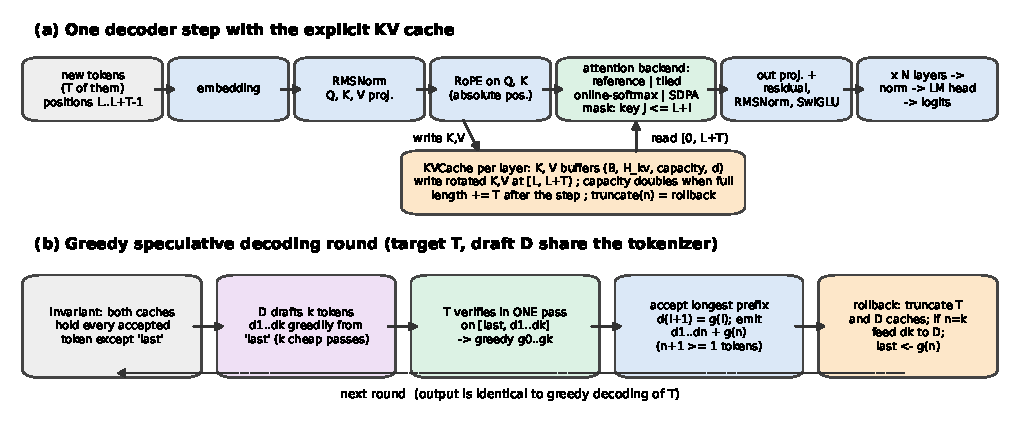
\includegraphics[width=.95\textwidth]{fig_decoder.pdf}
\caption{Architecture of our decoder implementation. (a) One forward step with the explicit, growable KV cache and the pluggable attention back-end (reference, tiled online-softmax, or PyTorch SDPA for comparison). (b) One round of greedy speculative decoding with cache rollback; the output equals greedy decoding of the target.}\label{fig:decoder}\end{figure*}

\emph{Positions.} Rotary embeddings rotate each query and key by its absolute position. For a step that feeds $T$ new tokens after $L$ cached ones, positions are $L,\dots,L+T-1$. Keys are rotated \emph{before} they are written to the cache, so cached keys already carry their position and are never rotated again; queries are rotated the same way and never cached.

\emph{Masking.} Query $i$ of the new block has absolute position $L+i$ and may attend to cache entry $j$ iff $j\le L+i$. During prefill ($L=0$) this is the usual lower-triangular mask; during one-token decoding ($T=1$) it admits the entire cache. The same \texttt{q\_offset} argument drives the mask in all attention back-ends.

\emph{Growth and rollback.} Each layer owns a pre-allocated key tensor and value tensor of shape $(B,H_{kv},C,d)$ with a shared length counter. New keys/values are written at slots $[L,L+T)$; if $L+T>C$ the capacity doubles (amortised $O(1)$ copies per token, in contrast to one \texttt{torch.cat} per step). Rolling back $n$ tokens is just setting the counter to $L-n$, which later writes overwrite---this is exactly what speculative decoding needs. With 32 layers, 5 KV heads and $d=64$, one cached token costs $2\cdot32\cdot5\cdot64\cdot4=82{,}000$ bytes in fp32 (about 80\,KB), i.e.\ 3$\times$ less than with 15 KV heads.

\emph{Numerical differences.} Cached and uncached paths compute the same mathematical function but with different matrix shapes (e.g.\ a $1\times d$ query against $L$ keys versus a full $T\times T$ product), which changes floating-point summation order. Logits can therefore differ at the $10^{-5}$ level, and a greedy argmax can flip only when the top-two logits are closer than that. We test token equality empirically (Section~\ref{sec:kvres}).

\subsection{Reference and Tiled Online-Softmax Attention}
\label{sec:attn}
The reference routine computes $S=QK^\top/\sqrt d$, applies the causal mask $M_{ij}=[j\le i+L]$ by setting masked scores to $-\infty$, subtracts the row maximum, exponentiates, normalises and multiplies by $V$; fully masked rows return zeros instead of NaN.

The tiled routine (Algorithm~\ref{alg:tiled}) never forms $S$. For each block of queries it sweeps over blocks of keys while keeping per-row statistics: the running maximum $m$, the running normaliser $\ell=\sum_j e^{s_j-m}$ and the running un-normalised output $o=\sum_j e^{s_j-m}v_j$. When a new key block with block maximum $\tilde m$ arrives, $m'=\max(m,\tilde m)$, the old statistics are rescaled by $\alpha=e^{m-m'}$, and the new block's contributions are added with the new maximum. The final output is $o/\ell$. Key blocks entirely above the causal diagonal are skipped, and grouped KV heads are broadcast to query heads block by block. PyTorch's fused \texttt{scaled\_dot\_product\_attention} is used only as a third comparison point.

\begin{algorithm}[t]\caption{Tiled attention with online softmax (one head)}\label{alg:tiled}
\begin{algorithmic}[1]
\small
\For{each query block $Q_b$ (rows $r$)}
 \State $m\gets-\infty,\ \ell\gets0,\ o\gets0$
 \For{each key block $K_c,V_c$ with $c$ not strictly above the diagonal}
  \State $S\gets Q_bK_c^\top/\sqrt d$; mask entries with key position $>$ query position
  \State $m'\gets\max(m,\mathrm{rowmax}(S))$;\ \ $\alpha\gets e^{m-m'}$;\ \ $P\gets e^{S-m'}$
  \State $\ell\gets\alpha\ell+\mathrm{rowsum}(P)$;\ \ $o\gets\alpha o+PV_c$;\ \ $m\gets m'$
 \EndFor
 \State output rows $\gets o/\ell$
\EndFor
\end{algorithmic}
\end{algorithm}

\subsection{Greedy Speculative Decoding}
\label{sec:spec}
Target (360M) and draft (135M) share the tokenizer, so token IDs are directly comparable. Both are held to one invariant at the start of each round: \emph{both caches contain every accepted token except the most recent one} ($\mathit{last}$). A round (Algorithm~\ref{alg:spec}) (1) lets the draft decode $k$ tokens from $\mathit{last}$, (2) runs \emph{one} target forward pass over $[\mathit{last},d_1,\dots,d_k]$, whose output at position $i$ is the target's greedy token $g_i$ after the $i$-th input, (3) accepts the longest prefix with $d_{i+1}=g_i$ and appends the target's own token $g_n$ (a correction at the first mismatch, or a free bonus token if all $k$ matched), and (4) restores the invariant: the target cache is truncated to keep only $\mathit{last},d_1..d_n$; the draft cache is truncated likewise, or, if all drafts were accepted, receives $d_k$ (which it had generated but never consumed). Each round therefore emits $n+1\ge1$ tokens and, by construction, the output equals greedy decoding of the target.

\begin{algorithm}[t]\caption{One round of greedy speculative decoding}\label{alg:spec}
\begin{algorithmic}[1]
\small
\State $d_1..d_k\gets$ draft greedy tokens starting from $\mathit{last}$ (draft cache grows by $k$)
\State $g_0..g_k\gets\arg\max$ of target logits on $[\mathit{last},d_1..d_k]$ (target cache grows by $k{+}1$)
\State $n\gets$ largest $n\le k$ with $d_i=g_{i-1}\ \forall i\le n$
\State emit $d_1..d_n,g_n$;\ \ target cache $\gets$ keep $\mathit{last},d_1..d_n$
\If{$n=k$} feed $d_k$ to the draft \Else{} truncate draft cache to $\mathit{last},d_1..d_n$ \EndIf
\State $\mathit{last}\gets g_n$
\end{algorithmic}
\end{algorithm}

\subsection{Criterion-Level Pipeline and Aggregation}
Fig.~\ref{fig:system} gives the end-to-end system: the offline training path (dataset, fixed split, prompt construction, LoRA fine-tuning, adapter selection) and the inference path used by the evaluation scripts and the browser application (input validation and sentence numbering, our decoder with the merged adapter under a chosen decoding mode, parsing, evidence extraction and explanation, rule-based aggregation, comparison view and report export).

\begin{figure*}[t]\centering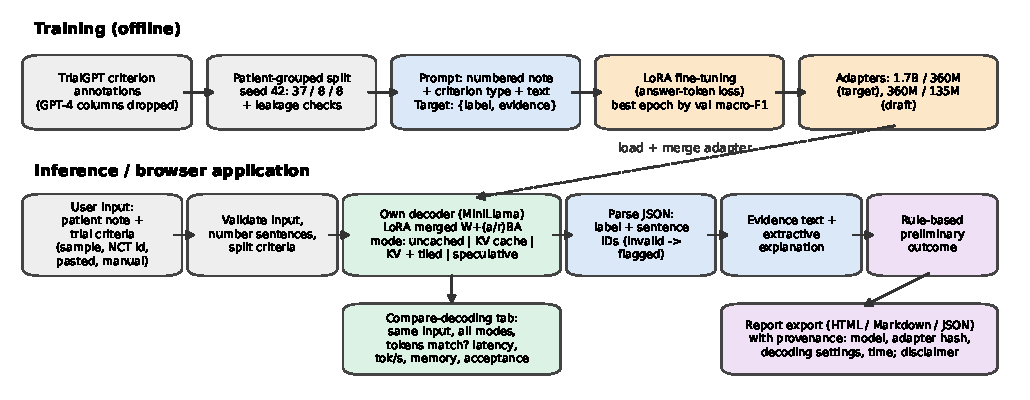
\includegraphics[width=.95\textwidth]{fig_system.pdf}
\caption{System architecture and application workflow. Top: offline training with the prescribed dataset and fixed split. Bottom: inference as used by evaluation and by the browser application.}\label{fig:system}\end{figure*}

For every criterion the pipeline returns: the criterion, predicted label, cited sentence IDs (IDs absent from the note are discarded and reported), the extracted text of those sentences, and an explanation. The explanation is a deterministic template that restates the label and quotes only the cited sentences; for \emph{not enough information} it states that missing mention is not evidence either way. We deliberately do not train on or generate free-text rationales, because the only rationales in the corpus are GPT-4 outputs that the protocol forbids. A patient--trial \emph{preliminary outcome} is an explicit rule over the criterion labels, not a learned or ground-truth label: any inclusion \emph{not included} or exclusion \emph{excluded} gives ``likely not eligible''; otherwise any \emph{not enough information} or invalid output gives ``needs more information''; otherwise ``potentially eligible''.

\subsection{Application}
\label{sec:app}
The application (FastAPI back-end, single-page browser UI, \texttt{app/}) loads the target and draft once, then lets a user paste a note (auto-numbered when needed), choose a held-out sample trial, fetch one from ClinicalTrials.gov by NCT ID (metadata only), or paste an eligibility block that is split into criteria. It shows each criterion's label, cited sentences highlighted in the numbered note, the explanation and raw output, and a rule-based overall outcome; reports are exported as HTML, Markdown or JSON with model, adapter hash, decoding settings and time stamp. A \emph{Compare decoding} tab runs the current input through all four decoding modes on the user's machine and tabulates tokens-match, latency, throughput, memory and acceptance rate; an \emph{Experiments} tab renders the stored result files. Invalid input (short notes, unknown criterion types, empty reports, unreachable trial registry) is rejected with explanatory messages. A banner states that this is an educational screening prototype and not a clinical enrollment decision.

\section{Experimental Setup and Metrics}

\subsection{Compute Environment and Memory Limits}
\textbf{Configuration~A (GPU)} ran on a free Kaggle notebook with one NVIDIA Tesla T4 (15\,GB; the notebook exposes two, only one is used), PyTorch~2.11 (CUDA~13 build), a recent Hugging Face Transformers~5.x~\cite{wolf2020transformers} and PEFT~0.21 for training and for reference checks. Training used fp16 autocast with fp32 master weights and LoRA parameters; \emph{all inference, evaluation and benchmarks run in fp32} so that exact-equality tests are meaningful. The 1.7B target needs about 6.85\,GB for fp32 weights, which together with activations left too little room for a micro-batch of 4 on the first attempt (an out-of-memory error), hence micro-batch 1 with 16 accumulation steps.

\textbf{Configuration~B (CPU)} ran on a laptop: Intel Core i5-1135G7 (4 cores / 8 threads), 16\,GB RAM, Windows~11, no GPU, PyTorch~2.14 (CPU build), Transformers~5.22 and PEFT~0.21. Everything uses fp32 on four threads, because CPU bf16 matrix multiplication is slower than fp32 on this processor and would add rounding noise to the exact-equality tests. The 360M target needs roughly 1.45\,GB for weights and, during LoRA training with activations and AdamW state, a peak working set of about 4\,GB; the 135M draft needs about 0.55\,GB. Training time on this machine is the practical limit that fixed the model size (Section~III-C).

Both configurations use exactly the same data split, prompts, parser, metrics and code; only the model pair, device and training schedule differ. The CPU configuration also serves as the model of the locally hosted application.

\subsection{Classification Metrics}
We report accuracy, macro-F1 and per-class precision, recall and F1 with support, plus confusion matrices, for all test criteria and separately for inclusion and exclusion criteria. Macro-F1 averages over the classes that occur either in the gold labels or in the predictions of the scope under consideration; a class absent from both is skipped, so the missing \emph{excluded} class in the test split does not silently count as a zero. An \emph{invalid} model output is counted as wrong and is never mapped onto a label. Because the test split contains only 8 patients whose rows are correlated, we also give 95\% patient-level bootstrap intervals (2\,000 resamples of patients).

\subsection{Evidence-Sentence Metrics}
Evidence is scored on sentence IDs as set overlap. \emph{Micro} scores pool true/false positives and false negatives over all records. \emph{Macro} scores average per-record precision, recall and F1 in two ways: (a) over records with at least one gold sentence (``evidence-bearing''), where predicting nothing yields precision 0 by convention, and (b) over all records, where an empty gold set matched by an empty prediction counts as a perfect record. Records with empty gold evidence are additionally reported on their own: the fraction for which the model also cited nothing and the number of spurious citations it made. About \NGoldEmpty{} of the \NGoldNon{}+\NGoldEmpty{} test records have no annotated evidence, so the policy matters and we show both views. Absence of cited evidence is never converted into an eligibility judgement.

\subsection{Decoding Settings}
Every accuracy number uses deterministic greedy decoding (argmax), at most 48 new tokens, stopping at the end-of-turn token, with the same prompt for the base and the adapted model. The base model is evaluated zero-shot with the identical prompt and parser on exactly the same validation and test rows; it receives no few-shot examples and no adapter. Hyper-parameters were chosen once from the configuration in Section~III-D and not tuned on the test split.

\subsection{Inference Benchmarks}
\emph{KV cache.} For prompt lengths $\{64,256,512\}$ tokens (real prompts built from test criteria, concatenated and cut) and output lengths $\{16,64,128\}$, the uncached reference, the cached path and the cached path with the tiled kernel generate with EOS suppressed so that all paths emit exactly the same number of tokens. These benchmarks were run on the GPU of Configuration~A (1.7B target); the laptop CPU was used for training, evaluation and the live comparison inside the application (Section~\ref{sec:appres}), not for stored benchmark tables. Each benchmark point runs in a fresh process with one warm-up generation and three timed repetitions; we report medians of prefill time (time to the first token), decode time, tokens per second and peak memory growth. On the GPU the memory figure is the exact CUDA-allocator peak minus the allocation before the call (\texttt{torch.cuda.max\_memory\_allocated}); in the application on a CPU it is the resident-set size sampled every 2\,ms while generating (peak minus the value before the call), a proxy because the CPU allocator has no peak counter. Greedy token sequences must be identical across paths.

\emph{Attention.} Shapes follow the 360M model (15 query heads, 5 KV heads, $d=64$) for $T\in\{128,\dots,4096\}$ on the GPU, in prefill mode ($T_q=T_k=T$) and decode mode ($T_q=1$ against $T$ cached keys), with five repetitions per point and the same fresh-process memory probe. Errors are the maximum and mean absolute difference to the reference output.

\emph{Speculative decoding.} Thirty-two test-criterion prompts (sampled with a fixed seed; only speed and token equality are measured, no model selection uses them) are decoded by cached greedy target decoding and by our speculative decoder for $k\in\{2,4,6,8\}$, once with the LoRA-adapted draft and once with the un-adapted draft. We report token equality, acceptance rate (accepted drafted tokens / drafted tokens), mean accepted tokens per round, target passes per emitted token, mean latency, tokens per second and speed-up. Two output regimes are used: the \emph{natural} task output (about 15 tokens of JSON) and a \emph{forced} 64-token output (EOS suppressed) that exposes behaviour on longer generations. Hugging Face assisted generation serves as an independent equality check on a subset.

\section{Results and Discussion}
\label{sec:results}
We report two configurations that use the identical split, prompt, parser and metrics. \textbf{Configuration~A} (GPU, Kaggle T4) fine-tunes SmolLM2-1.7B as target with SmolLM2-360M as draft and carries the headline accuracy results; \textbf{Configuration~B} (CPU, laptop) uses the 360M target with the 135M draft and is the model that the locally hosted application loads by default (Section~\ref{sec:cpu}). All numbers below come from files written by the scripts in the repository.

\subsection{Fine-Tuning and Model Selection (Config.~A)}
Table~\ref{tab:epochsA} lists validation behaviour after each epoch and Fig.~\ref{fig:trainA} the training curves. Answer-token training loss falls from about 0.40 to about 0.12 for the 1.7B target, and validation loss falls from 0.190 to 0.155 between epochs 1 and 2 and then stays flat (0.156). Validation macro-F1 peaks at epoch \GTBestEpoch{} (0.365) and drops at epoch 3 (0.326), and validation accuracy follows the same pattern (0.714 vs.\ 0.694), so the epoch-2 adapter was kept for the target; the same criterion selected epoch \GDBestEpoch{} for the 360M draft (Table~\ref{tab:epochsAd}). Because macro-F1 over six classes on 206 validation rows is noisy (the curves in Fig.~\ref{fig:trainA} move by several points between epochs while the loss is flat), the selection is made on a weak signal; we report it as observed rather than as a tuned optimum. Training took \GTTrainHours{}\,h (target) and \GDTrainHours{}\,h (draft) on one T4 with fp16 autocast, micro-batch 1 and 16 accumulation steps for the 1.7B model (to fit 15\,GB), and micro-batch 4 with 4 accumulation steps for the draft; the effective batch is 16 in both cases.

\begin{table}[t]\centering\caption{Config.~A target (SmolLM2-1.7B + LoRA): validation after each epoch ($^*$ = selected).}\label{tab:epochsA}
\small\begin{tabular}{rrrrr}\toprule
Epoch & Val. loss & Val. acc. & Val. macro-F1 & Val. evid. F1 \\\midrule
1 & 0.190 & 0.675 & 0.309 & 0.306 \\
2$^*$ & 0.155 & 0.714 & 0.365 & 0.374 \\
3 & 0.156 & 0.694 & 0.326 & 0.391 \\
\bottomrule\end{tabular}
\end{table}
\begin{table}[t]\centering\caption{Config.~A draft (SmolLM2-360M + LoRA): validation after each epoch.}\label{tab:epochsAd}
\small\begin{tabular}{rrrrr}\toprule
Epoch & Val. loss & Val. acc. & Val. macro-F1 & Val. evid. F1 \\\midrule
1 & 0.220 & 0.621 & 0.215 & 0.124 \\
2$^*$ & 0.192 & 0.718 & 0.341 & 0.325 \\
3 & 0.186 & 0.641 & 0.259 & 0.063 \\
4 & 0.184 & 0.689 & 0.323 & 0.262 \\
\bottomrule\end{tabular}
\end{table}
\begin{figure}[t]\centering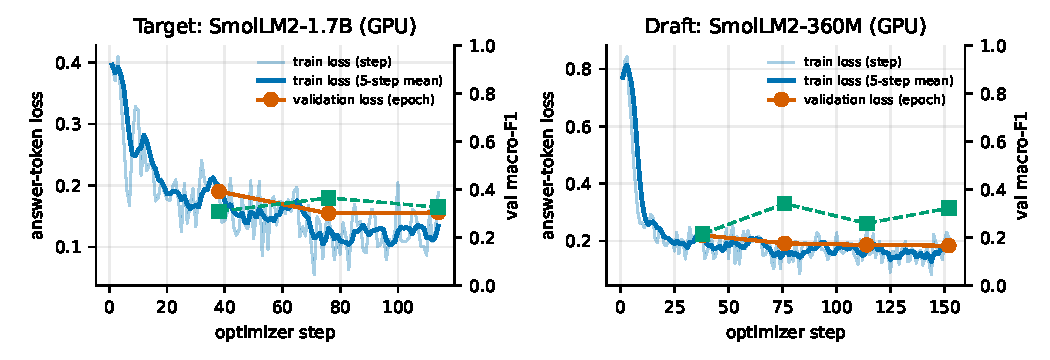
\includegraphics[width=\columnwidth]{gpu_fig_training.pdf}
\caption{Config.~A training curves: step and smoothed training loss, epoch-level validation loss (red) and validation macro-F1 (green, right axis).}\label{fig:trainA}\end{figure}

\subsection{Before and After Fine-Tuning (Config.~A)}
Table~\ref{tab:mainA} compares, on \emph{identical} validation and test rows with the same prompt, greedy decoding and parser, a trivial majority-label baseline, the base model used zero-shot, and the fine-tuned model; Fig.~\ref{fig:baA} visualises the test columns. The base model is almost never right: test accuracy \GBaseAcc{} (95\% patient-bootstrap interval \GBaseAccLo--\GBaseAccHi) and macro-F1 \GBaseMF{}. Its outputs are well-formed JSON (only \GBaseInvalid{} invalid output), so the failure is semantic: it commits to a decisive label, and on all 131 exclusion rows it never produces the correct one (exclusion accuracy 0.000). Fine-tuning lifts test accuracy to \GTestAcc{} (interval \GTestAccLo--\GTestAccHi) and macro-F1 to \GTestMF{} (interval \GTestMFLo--\GTestMFHi), with no invalid outputs.

Two cautions are needed to read this correctly. First, a trivial predictor already attains \GMajAcc{} accuracy on the test split because \emph{not excluded} and \emph{not enough information} dominate; the accuracy interval of the fine-tuned model (lower end \GTestAccLo) therefore overlaps the majority baseline, so we cannot claim a statistically supported accuracy gain over guessing the common label. The macro-F1 gain is clearer (0.460 vs.\ 0.272, interval lower end \GTestMFLo), because macro-F1 rewards the minority classes. Second, the gain is entirely on inclusion criteria: inclusion accuracy rises from the majority baseline's 0.507 to 0.747 and macro-F1 from 0.168 to 0.516, whereas exclusion accuracy (0.687) is \emph{below} the majority baseline's 0.695 and macro-F1 is unchanged (0.271 vs.\ 0.273). The reason is visible in the confusion matrices below: for exclusion criteria the model predicts \emph{not excluded} for 130 of 131 rows.

\begin{table*}[t]\centering\caption{Config.~A: majority baseline, base zero-shot and fine-tuned SmolLM2-1.7B on the same rows (acc.\ = accuracy, mF1 = macro-F1; Invalid = unparseable outputs).}\label{tab:mainA}
\small\begin{tabular}{llrrrrrrr}\toprule
Split & Model & Acc. & mF1 & Incl. acc. & Incl. mF1 & Excl. acc. & Excl. mF1 & Invalid \\\midrule
Val. & majority label & 0.621 & 0.215 & 0.409 & 0.145 & 0.721 & 0.210 & 0 \\
& base zero-shot & 0.170 & 0.131 & 0.500 & 0.206 & 0.014 & 0.007 & 0 \\
& fine-tuned & 0.714 & 0.365 & 0.667 & 0.344 & 0.736 & 0.269 & 0 \\
\midrule
Test & majority label & 0.626 & 0.272 & 0.507 & 0.168 & 0.695 & 0.273 & 0 \\
& base zero-shot & 0.146 & 0.111 & 0.400 & 0.182 & 0.000 & 0.000 & 1 \\
& fine-tuned & 0.709 & 0.460 & 0.747 & 0.516 & 0.687 & 0.271 & 0 \\
\bottomrule\end{tabular}
\end{table*}
\begin{figure}[t]\centering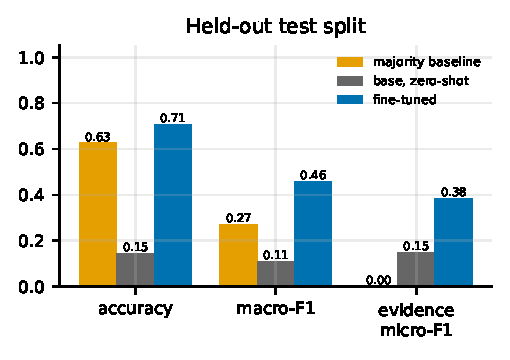
\includegraphics[width=.8\columnwidth]{gpu_fig_before_after.pdf}
\caption{Config.~A test results: majority baseline, base zero-shot and fine-tuned model.}\label{fig:baA}\end{figure}

\subsection{Per-Class Results and Inclusion vs.\ Exclusion (Config.~A)}
Table~\ref{tab:pcA} and Fig.~\ref{fig:cmA} give per-class precision, recall and F1 and the confusion matrices overall and by criterion type (rows are expert labels, columns predictions). \emph{Included} is handled well (P 0.79, R 0.70, F1 0.75 on 27 rows) and \emph{not excluded} has high recall (0.99) but only 0.69 precision because 28 \emph{not enough information} and 12 \emph{not applicable} exclusion rows are also labelled \emph{not excluded}. \emph{Not enough information} reaches F1 0.62 (inclusion: 36 of 38 correct), \emph{not applicable} has precision 1.0 but recall 0.07 (1 of 15), and \emph{not included} (7 rows) is never predicted. The \emph{excluded} class has no test support, so it contributes neither to recall nor to macro-F1 (Section~IV-B). The base model's per-class table (Table~\ref{tab:pcB}) shows the contrast: it spreads predictions over decisive labels with near-zero precision. Table~\ref{tab:pcA} should therefore be read as: reliable on \emph{included} and \emph{not enough information} for inclusion criteria, essentially majority-class behaviour for exclusion criteria, and no ability on the rarest classes.

\begin{table}[t]\centering\caption{Config.~A fine-tuned model, test split: per-class precision (P), recall (R), F1 and support.}\label{tab:pcA}
\footnotesize\begin{tabular}{llrrrr}\toprule
Scope & Class & P & R & F1 & Support \\\midrule
inclusion & included & 0.792 & 0.704 & 0.745 & 27 \\
 & not included & 0.000 & 0.000 & 0.000 & 7 \\
 & not enough info. & 0.720 & 0.947 & 0.818 & 38 \\
 & not applicable & 1.000 & 0.333 & 0.500 & 3 \\
\midrule
exclusion & excluded & 0.000 & 0.000 & 0.000 & 0 \\
 & not excluded & 0.692 & 0.989 & 0.814 & 91 \\
 & not enough info. & 0.000 & 0.000 & 0.000 & 28 \\
 & not applicable & 0.000 & 0.000 & 0.000 & 12 \\
\bottomrule\end{tabular}
\end{table}
\begin{table}[t]\centering\caption{Config.~A base model (zero-shot), test split.}\label{tab:pcB}
\footnotesize\begin{tabular}{llrrrr}\toprule
Scope & Class & P & R & F1 & Support \\\midrule
inclusion & included & 0.409 & 1.000 & 0.581 & 27 \\
 & not included & 0.000 & 0.000 & 0.000 & 7 \\
 & not enough info. & 1.000 & 0.079 & 0.146 & 38 \\
 & not applicable & 0.000 & 0.000 & 0.000 & 3 \\
\midrule
exclusion & excluded & 0.000 & 0.000 & 0.000 & 0 \\
 & not excluded & 0.000 & 0.000 & 0.000 & 91 \\
 & not enough info. & 0.000 & 0.000 & 0.000 & 28 \\
 & not applicable & 0.000 & 0.000 & 0.000 & 12 \\
\bottomrule\end{tabular}
\end{table}
\begin{figure*}[t]\centering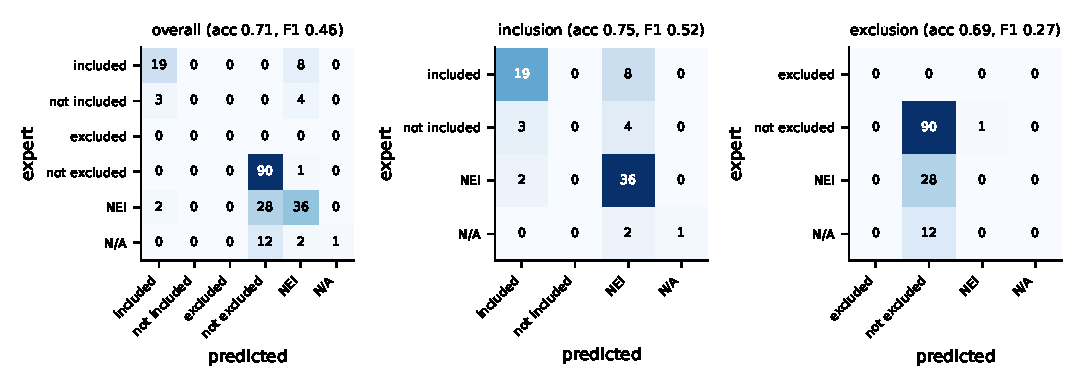
\includegraphics[width=.85\textwidth]{gpu_fig_confusion.pdf}
\caption{Config.~A confusion matrices on the test split (NEI = not enough information, N/A = not applicable).}\label{fig:cmA}\end{figure*}

\subsection{Evidence-Sentence Localisation (Config.~A)}
Table~\ref{tab:evA} reports sentence-ID precision, recall and F1. \NGoldEmpty{} of the \NTest{} test records have \emph{no} annotated evidence sentence and only \NGoldNon{} have at least one, which dominates every aggregate. With micro pooling the fine-tuned model reaches P~0.538, R~0.298, F1~\GTestEvF{} (interval \GTestEvFLo--\GTestEvFHi) against the base model's 0.151: the base model cites many sentences (recall 0.447, precision 0.091), the adapted model cites few but more correct ones. On evidence-bearing records the macro F1 is 0.277; if empty-gold records count as correct when nothing is cited, macro F1 rises to 0.757 purely because the model leaves 95.9\% of the empty-gold records empty (10 spurious citations in total), which shows why that second number must not be read as localisation skill. The split by type is telling: inclusion micro-F1 is 0.491 while exclusion micro-F1 is 0.000, because the model never cites a sentence for an exclusion criterion. Cited IDs are always valid sentence IDs of the note, and the application only displays text that exists in the note.

\begin{table}[t]\centering\caption{Config.~A evidence-sentence metrics on the test split (micro, and macro over evidence-bearing or all records).}\label{tab:evA}
\footnotesize\setlength{\tabcolsep}{3pt}\resizebox{\columnwidth}{!}{\begin{tabular}{llrrrr}\toprule
Model & Scope & P & R & F1 & Type \\\midrule
base & overall & 0.091 & 0.447 & 0.151 & micro \\
base & inclusion & 0.158 & 0.500 & 0.240 & micro \\
base & exclusion & 0.041 & 0.344 & 0.074 & micro \\
base & overall & 0.267 & 0.412 & 0.295 & macro (gold$\neq\emptyset$) \\
base & overall & 0.079 & 0.122 & 0.087 & macro (all records) \\\midrule
fine-tuned & overall & 0.538 & 0.298 & 0.384 & micro \\
fine-tuned & inclusion & 0.538 & 0.452 & 0.491 & micro \\
fine-tuned & exclusion & 0.000 & 0.000 & 0.000 & micro \\
fine-tuned & overall & 0.290 & 0.295 & 0.277 & macro (gold$\neq\emptyset$) \\
fine-tuned & overall & 0.761 & 0.762 & 0.757 & macro (all records) \\\bottomrule\end{tabular}
}\end{table}

\subsection{Error Analysis (Config.~A)}
\label{sec:errors}
Of the \NTest{} test criteria, \GNLabelErr{} (29\%) receive a wrong label and a further 35 have a correct label with a different evidence set; 111 are correct in both respects. Table~\ref{tab:errcatA} categorises every non-correct case and Table~\ref{tab:errA} lists twelve representative, distinct cases from different patients, trials and categories (full text in \texttt{results/error\_analysis\_gpu\_finetuned\_test.md}).

\emph{Missing information treated as ``not excluded''.} The largest category is false decision: 42 rows whose expert label is \emph{not enough information} (30) or \emph{not applicable} (12) but where the model commits to a decisive label; 40 of the 42 are exclusion criteria answered \emph{not excluded}. E1 (``Pregnancy'', expert: not applicable) and E3 (``BMI $>$ 40'', expert: not enough information) are typical: the note contains nothing about the topic and the model, instead of reporting the gap, defaults to the label that is correct most often. This is exactly the behaviour the task warns against---absence of evidence being read as eligibility---so \emph{not excluded} outputs without cited evidence should be shown to users as unverified, which the application does by displaying ``no supporting sentence cited''.

\emph{Uncited decisive predictions.} 130 test predictions carry a decisive label with no cited sentence. For 114 of them the expert also cites nothing, which is consistent with the dataset (about three quarters of \emph{not excluded} labels have empty evidence), but 16 have expert evidence that the model failed to cite (E4, E8): these are the contradictory cases where a label is given without the supporting sentence that exists in the note.

\emph{Missed decisions.} 13 rows have a decisive expert label but the model answers \emph{not enough information} (E7, E8): for example ``Shock or ARDS'' is marked \emph{included} by the expert based on hypotension and tachycardia (sentences 2--3), while the model says the note lacks information. These failures need clinical inference from vital signs, which a small model trained on 602 rows does not acquire.

\emph{Polarity flips and \emph{not applicable} confusions} are rare (3 and 2), and the \emph{not included} class (7 rows) is mostly answered \emph{included} (3) or \emph{not enough information} (4). \emph{Evidence-only} errors (35) divide into over-citation, where a \emph{not enough information} answer cites the first five sentences although the expert cites none (E5), and under-citation, where the single relevant sentence is missed (E6).

\begin{table}[t]\centering\caption{Config.~A test errors by category (all 206 rows; ``correct'' means label and evidence both match).}\label{tab:errcatA}
\small\begin{tabular}{lr}\toprule
Error category & Count \\\midrule
correct & 111 \\
false decision & 42 \\
evidence only & 35 \\
missed decision & 13 \\
polarity flip & 3 \\
na confusion & 2 \\
\bottomrule\end{tabular}
\end{table}
\begin{table*}[t]\centering\caption{Config.~A: twelve representative errors (evidence lists are sentence IDs; Expert/Model columns show label and IDs).}\label{tab:errA}
\scriptsize\begin{tabular}{p{.05\linewidth}p{.15\linewidth}p{.32\linewidth}p{.13\linewidth}p{.13\linewidth}}\toprule
ID & Type & Criterion (abridged) & Expert & Model \\\midrule
E1 & false decision & Pregnancy & not applicable [] & not excluded [] \\
E2 & false decision & Patients were moribund. & not enough info. [0, 1, 2, 3, 4] & not excluded [] \\
E3 & false decision & BMI> 40 kg/m2. & not enough info. [] & not excluded [] \\
E4 & evidence only & Had been performed central venous puncture or catheterization before. & not excluded [0] & not excluded [] \\
E5 & evidence only & bilateral pulmonary infiltrates or a chest radiograph consistent with edema; & not enough info. [] & not enough info. [0, 1, 2, 3, 4] \\
E6 & evidence only & Patients with liver space occupying lesion (LOE) that require extended hepatic resection. & not enough info. [3] & not enough info. [] \\
E7 & missed decision & Patients undergoing elective carotid endarterectomy & not included [] & not enough info. [] \\
E8 & missed decision & Patients were included if they were diagnosed with Shock, Acute respiratory distress syndr… & included [2, 3] & not enough info. [] \\
E9 & missed decision & Present with active SLE disease with at least one of the following symptoms: i) Arthritis … & included [0, 1] & not enough info. [] \\
E10 & polarity flip & Patients undergoing open abdominal aortic aneurysm repair & not included [] & included [0] \\
E11 & na confusion & If female, using birth control & not applicable [3] & not enough info. [] \\
E12 & na confusion & female patients have adequate birth-control method & not applicable [] & not enough info. [] \\
\bottomrule\end{tabular}
\end{table*}

\subsection{KV-Cached Generation (Config.~A)}
\label{sec:kvres}
Table~\ref{tab:kvA} compares the uncached reference, the explicit KV cache with PyTorch SDPA attention, and the cache combined with our tiled kernel for prompts of 64, 256 and 512 tokens and 16, 64 and 128 generated tokens on the T4, in fp32 on the 1.7B model. \textbf{Correctness:} the greedy token sequences of all three paths are identical in \GKVAllMatch{} configurations, including 512+128 tokens, even though the cached path multiplies a single query against the cache while the reference recomputes full matrices; no mismatch needed investigation, and the unit tests on smaller models additionally match the Hugging Face logits to $6\times10^{-5}$. \textbf{Speed:} prefill time is the same for all paths (0.09--0.7\,s, growing with prompt length) as expected, because prefill computes the same thing. Decode is where the cache matters: the uncached path re-reads and recomputes the whole prefix at every step, so its throughput (prefill included) is only 4.3--6.6 tokens/s for 64-token prompts and falls to 1.2--1.3 tokens/s for 512-token prompts, whereas the cached path stays between 14 and 30 tokens/s, i.e.\ \GKVSpeedup$\times$ faster end to end at 512+128 tokens (Fig.~\ref{fig:kvtimeA}). The cached tokens/s itself declines mildly with prompt length (30.1 at 64 tokens to 24.8 at 512) because every step attends to more cached keys. \textbf{Memory:} the cache is the price paid for this speed. The 1.7B model uses multi-head attention with 32 KV heads, so one cached token costs $2\cdot24\cdot32\cdot64\cdot4=393$\,kB in fp32 (the measured 239.6\,MB for 639 tokens agrees), and the measured peak allocation growth is 289--331\,MB with the cache versus 91--110\,MB without at 512 tokens (Fig.~\ref{fig:kvmemA}); this includes the pre-allocated buffer of 256 or more slots. For comparison, the grouped-query 360M model needs only 82\,kB per token. \textbf{Tiled attention inside the decoder:} the cached path with our tiled kernel produces identical tokens but is 1.6--4.5$\times$ slower than SDPA (5.5 vs.\ 24.8 tokens/s at 512+128) because every decode step runs a Python loop over key blocks, an overhead discussed next.

\begin{table*}[t]\centering\caption{Config.~A KV-cache benchmark (median of 3 repetitions after warm-up; peak $\Delta$ is the CUDA allocator peak above the pre-call level, KV = cache bytes in use; the last column checks token equality with the uncached reference).}\label{tab:kvA}
\small\begin{tabular}{rrlrrrrrc}\toprule
In & Out & Mode & Prefill (s) & Decode (s) & tok/s & Peak $\Delta$ (MB) & KV (MB) & = ref. \\\midrule
64 & 16 & uncached & 0.102 & 2.325 & 6.6 & 14 & 0.0 & yes \\
 &  & kv\_cache & 0.100 & 0.491 & 26.8 & 107 & 29.6 & yes \\
 &  & kv\_cache\_tiled & 0.094 & 0.884 & 16.4 & 107 & 29.6 & yes \\
64 & 64 & uncached & 0.125 & 12.331 & 5.1 & 22 & 0.0 & yes \\
 &  & kv\_cache & 0.089 & 2.024 & 30.2 & 107 & 47.6 & yes \\
 &  & kv\_cache\_tiled & 0.090 & 3.611 & 17.3 & 107 & 47.6 & yes \\
64 & 128 & uncached & 0.112 & 29.406 & 4.3 & 33 & 0.0 & yes \\
 &  & kv\_cache & 0.102 & 4.153 & 30.1 & 107 & 71.6 & yes \\
 &  & kv\_cache\_tiled & 0.105 & 8.277 & 15.3 & 107 & 71.6 & yes \\
256 & 16 & uncached & 0.327 & 6.490 & 2.3 & 47 & 0.0 & yes \\
 &  & kv\_cache & 0.334 & 0.511 & 18.9 & 149 & 101.6 & yes \\
 &  & kv\_cache\_tiled & 0.335 & 1.617 & 8.2 & 149 & 101.6 & yes \\
256 & 64 & uncached & 0.353 & 28.947 & 2.2 & 55 & 0.0 & yes \\
 &  & kv\_cache & 0.328 & 2.115 & 26.2 & 167 & 119.6 & yes \\
 &  & kv\_cache\_tiled & 0.351 & 6.659 & 9.1 & 167 & 119.6 & yes \\
256 & 128 & uncached & 0.347 & 60.917 & 2.1 & 66 & 0.0 & yes \\
 &  & kv\_cache & 0.328 & 4.308 & 27.6 & 191 & 143.6 & yes \\
 &  & kv\_cache\_tiled & 0.353 & 14.498 & 8.6 & 191 & 143.6 & yes \\
512 & 16 & uncached & 0.683 & 12.507 & 1.2 & 91 & 0.0 & yes \\
 &  & kv\_cache & 0.589 & 0.528 & 14.3 & 289 & 197.6 & yes \\
 &  & kv\_cache\_tiled & 0.669 & 2.623 & 4.9 & 289 & 197.6 & yes \\
512 & 64 & uncached & 0.656 & 49.965 & 1.3 & 99 & 0.0 & yes \\
 &  & kv\_cache & 0.612 & 2.217 & 22.6 & 307 & 215.6 & yes \\
 &  & kv\_cache\_tiled & 0.697 & 11.065 & 5.5 & 307 & 215.6 & yes \\
512 & 128 & uncached & 0.645 & 95.949 & 1.3 & 110 & 0.0 & yes \\
 &  & kv\_cache & 0.616 & 4.543 & 24.8 & 331 & 239.6 & yes \\
 &  & kv\_cache\_tiled & 0.714 & 22.456 & 5.5 & 331 & 239.6 & yes \\
\bottomrule\end{tabular}
\end{table*}
\begin{figure}[t]\centering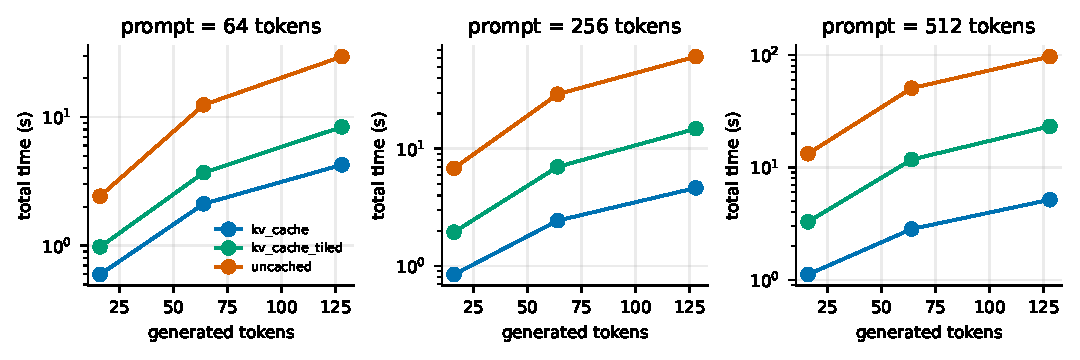
\includegraphics[width=\columnwidth]{gpu_fig_kv_time.pdf}
\caption{Config.~A: total generation time (log scale) against generated tokens for three prompt lengths.}\label{fig:kvtimeA}\end{figure}
\begin{figure}[t]\centering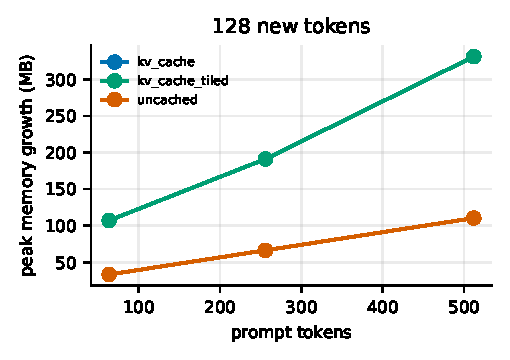
\includegraphics[width=.75\columnwidth]{gpu_fig_kv_memory.pdf}
\caption{Config.~A: peak allocation growth against prompt length at 128 new tokens.}\label{fig:kvmemA}\end{figure}

\subsection{Tiled Online-Softmax Attention (Config.~A)}
Table~\ref{tab:attnA} and Fig.~\ref{fig:attnA} validate and benchmark the kernels at the head shape of the 360M model (15 query heads, 5 KV heads, $d=64$) with random inputs. \textbf{Numerical agreement:} against the float32 reference the tiled kernel's maximum absolute error never exceeds $9.6\times10^{-7}$ across $T=128\ldots4096$ in prefill and $T=128\ldots2048$ in decode (worst error over all measured points, including SDPA: \GAttnWorstErr), with a mean error around $2\times10^{-8}$; unit tests add a hand-computed example, grouped heads, non-zero cache offsets, left padding and extreme score magnitudes where naive softmax overflows. \textbf{Memory:} the reference path's peak allocation grows quadratically (196\,MB at $T{=}1024$, 754\,MB at 2048, 2\,956\,MB at 4096) whereas the tiled kernel's grows roughly linearly (11, 22, 45\,MB), which is the intended effect of never forming the $T\times T$ score matrix. \textbf{Speed:} the tiled kernel is \emph{slower}: at $T{=}1024$ it needs 98\,ms against 5.9\,ms for the reference and 2.8\,ms for the fused SDPA kernel, and 1.6\,s against 83\,ms at 4096. This is expected for an educational PyTorch implementation: each tile launches half a dozen small kernels and Python-level loop iterations, reads and writes the running statistics from global memory, and cannot overlap data movement with compute as a fused FlashAttention-style kernel does with on-chip SRAM~\cite{dao2022flashattention}. The tile-size sweep supports this explanation (Fig.~\ref{fig:tileA}): at $T{=}1024$ the time drops from 1\,560\,ms with 16$\times$16 tiles to 98\,ms at 64, 30\,ms at 128 and 7.6\,ms at 256, nearly matching the reference, while the error is unchanged ($\le 9.5\times10^{-7}$)---the number of Python-level iterations, not arithmetic, dominates. In decode mode ($T_q{=}1$) there is no score matrix to save, so the reference (0.65\,ms) is even faster than SDPA (1.04\,ms) at $T{=}2048$, since both are launch-bound.

\begin{table}[t]\centering\caption{Config.~A attention benchmark: prefill ($T_q{=}T_k{=}T$) and decode ($T_q{=}1$) for three lengths; tiled uses 64$\times$64 tiles; errors are versus the reference.}\label{tab:attnA}
\footnotesize\setlength{\tabcolsep}{2.5pt}\resizebox{\columnwidth}{!}{\begin{tabular}{llrrrrr}\toprule
Phase & Impl. & $T$ & Time (ms) & Max err. & Mean err. & Peak $\Delta$ (MB) \\\midrule
prefill & reference & 256 & 1.01 & 0.0e+00 & 0.0e+00 & 15 \\
prefill & sdpa & 256 & 0.47 & 6.6e-07 & 3.1e-08 & 4 \\
prefill & tiled & 256 & 7.58 & 6.0e-07 & 2.7e-08 & 4 \\
prefill & reference & 1024 & 5.86 & 0.0e+00 & 0.0e+00 & 196 \\
prefill & sdpa & 1024 & 2.77 & 7.2e-07 & 3.0e-08 & 20 \\
prefill & tiled & 1024 & 98.06 & 8.3e-07 & 2.3e-08 & 11 \\
prefill & reference & 2048 & 20.25 & 0.0e+00 & 0.0e+00 & 754 \\
prefill & sdpa & 2048 & 12.13 & 6.9e-07 & 2.9e-08 & 50 \\
prefill & tiled & 2048 & 401.02 & 4.8e-07 & 2.2e-08 & 22 \\
\midrule
decode & reference & 256 & 0.67 & 0.0e+00 & 0.0e+00 & 2 \\
decode & sdpa & 256 & 0.36 & 1.5e-07 & 2.9e-08 & 2 \\
decode & tiled & 256 & 3.09 & 7.5e-08 & 1.1e-08 & 1 \\
decode & reference & 1024 & 0.66 & 0.0e+00 & 0.0e+00 & 8 \\
decode & sdpa & 1024 & 0.82 & 1.6e-07 & 2.6e-08 & 8 \\
decode & tiled & 1024 & 12.01 & 6.0e-08 & 9.5e-09 & 1 \\
decode & reference & 2048 & 0.65 & 0.0e+00 & 0.0e+00 & 15 \\
decode & sdpa & 2048 & 1.04 & 1.7e-07 & 2.4e-08 & 15 \\
decode & tiled & 2048 & 25.14 & 6.0e-08 & 9.2e-09 & 1 \\
\bottomrule\end{tabular}
}\end{table}
\begin{figure*}[t]\centering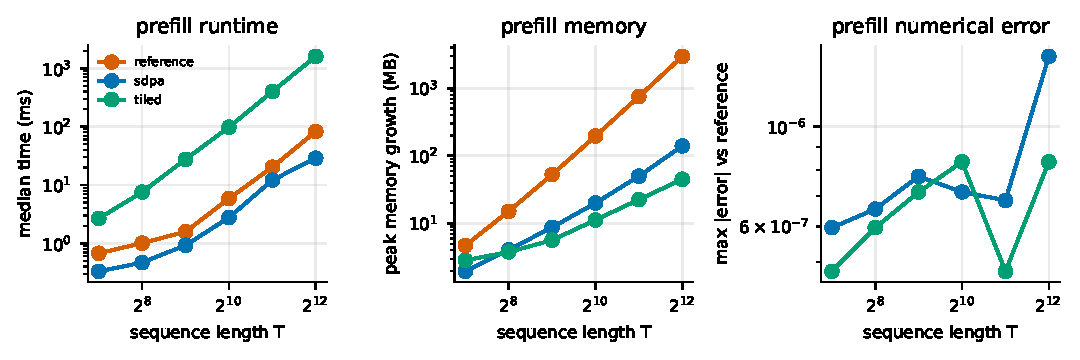
\includegraphics[width=.9\textwidth]{gpu_fig_attention.pdf}
\caption{Config.~A prefill attention: runtime, memory and error versus sequence length (log scales).}\label{fig:attnA}\end{figure*}
\begin{figure}[t]\centering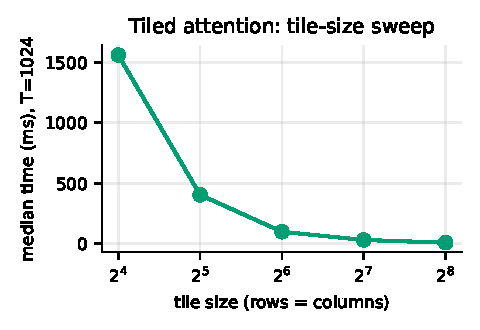
\includegraphics[width=.7\columnwidth]{gpu_fig_tile_sweep.pdf}
\caption{Config.~A: effect of tile size on tiled-attention time at $T=1024$.}\label{fig:tileA}\end{figure}

\subsection{Speculative Decoding (Config.~A)}
\label{sec:specres}
Tables~\ref{tab:specA1} and~\ref{tab:specA2} and Fig.~\ref{fig:specA} (acceptance and speed-up against the draft length $k$) compare cached greedy decoding of the 1.7B target against our speculative decoder with the fine-tuned 360M draft and with the un-tuned 360M draft, on 32 test prompts (speed only; no model selection used these prompts). \textbf{Correctness:} outputs are token-identical to greedy target decoding for \emph{every} prompt and every setting (32/32 in all 16 rows), and an independent check with Hugging Face assisted generation on six prompts agrees: \GSpecHF. \textbf{Acceptance:} with natural task output (about 13 tokens of JSON) the fine-tuned draft is accepted 92--98\% of the time, against 40--64\% for the un-tuned draft, so adapting the draft on the same task raises acceptance by 30--50 points; with forced 64-token outputs, where the continuation after the JSON is unconstrained, acceptance drops to 33--65\% for both drafts and the benefit of adaptation disappears. Acceptance falls with the draft length $k$ in all cases. \textbf{Latency:} despite high acceptance, speculative decoding is \emph{slower} than plain greedy decoding in every configuration: the best speed-up is \GSpecBestSpeedup$\times$ ($k{=}\GSpecBestK$, \GSpecBestDraft) for natural output and as low as 0.39$\times$ for forced long output. The cause is the cost ratio. On a GPU single-token decoding is limited by per-layer kernel launches and memory latency, not by arithmetic, so latency is roughly proportional to depth; the 360M draft has \emph{32} layers while the 1.7B target has only \emph{24}, so a draft step costs about as much as a target step. The speed-up model of Leviathan et al.~\cite{leviathan2023speculative}, $(1-\alpha^{k+1})/((1-\alpha)(kc+1))$, with draft/target cost ratio $c\approx1$, is below one for any acceptance rate. Our measured mean accepted length per round (5.8 tokens for the fine-tuned draft at $k{=}8$ on natural output, 2.3--2.5 for the un-tuned draft and for forced output) confirms that verification works as designed---the target needs well under one forward pass per emitted token (0.31 for forced output at $k{=}8$)---while draft cost cancels the gain. A faster configuration would need a much shallower draft (fewer layers) or a larger target. Memory is not an issue (extra allocation growth about 240\,MB, similar to the plain cache).

\begin{table}[t]\centering\caption{Config.~A speculative decoding, natural task output (32 prompts; Equal = outputs identical to greedy target; Accept. = accepted / proposed draft tokens).}\label{tab:specA1}
\footnotesize\begin{tabular}{llrrrrr}\toprule
Draft & $k$ & Equal & Accept. & Latency (s) & tok/s & Speed-up \\\midrule
\multicolumn{2}{l}{greedy target} & -- & -- & 0.894 & 15.0 & 1.00 \\\midrule
finetuned draft & 2 & 32/32 & 97\% & 1.180 & 11.4 & 0.76 \\
finetuned draft & 4 & 32/32 & 98\% & 1.133 & 11.8 & 0.79 \\
finetuned draft & 6 & 32/32 & 96\% & 1.102 & 12.2 & 0.81 \\
finetuned draft & 8 & 32/32 & 92\% & 1.110 & 12.1 & 0.81 \\
untuned draft & 2 & 32/32 & 64\% & 1.340 & 10.0 & 0.67 \\
untuned draft & 4 & 32/32 & 58\% & 1.370 & 9.8 & 0.65 \\
untuned draft & 6 & 32/32 & 49\% & 1.480 & 9.1 & 0.60 \\
untuned draft & 8 & 32/32 & 40\% & 1.630 & 8.2 & 0.55 \\
\bottomrule\end{tabular}
\end{table}
\begin{table}[t]\centering\caption{Config.~A speculative decoding, forced 64-token output.}\label{tab:specA2}
\footnotesize\begin{tabular}{llrrrrr}\toprule
Draft & $k$ & Equal & Accept. & Latency (s) & tok/s & Speed-up \\\midrule
\multicolumn{2}{l}{greedy target} & -- & -- & 2.571 & 24.9 & 1.00 \\\midrule
finetuned draft & 2 & 32/32 & 65\% & 4.230 & 15.1 & 0.61 \\
finetuned draft & 4 & 32/32 & 49\% & 4.798 & 13.3 & 0.54 \\
finetuned draft & 6 & 32/32 & 39\% & 5.743 & 11.1 & 0.45 \\
finetuned draft & 8 & 32/32 & 33\% & 6.547 & 9.8 & 0.39 \\
untuned draft & 2 & 32/32 & 63\% & 4.304 & 14.9 & 0.60 \\
untuned draft & 4 & 32/32 & 52\% & 4.629 & 13.8 & 0.56 \\
untuned draft & 6 & 32/32 & 41\% & 5.543 & 11.5 & 0.46 \\
untuned draft & 8 & 32/32 & 33\% & 6.471 & 9.9 & 0.40 \\
\bottomrule\end{tabular}
\end{table}
\begin{figure*}[t]\centering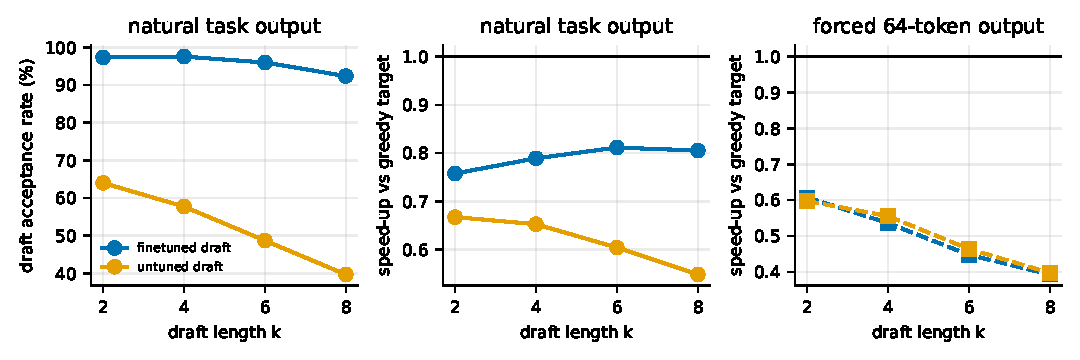
\includegraphics[width=.9\textwidth]{gpu_fig_speculative.pdf}
\caption{Config.~A: acceptance rate and speed-up against draft length $k$ for the fine-tuned and un-tuned draft.}\label{fig:specA}\end{figure*}

\subsection{Configuration B: CPU Laptop Model}
\label{sec:cpu}
Configuration~B repeats the experiment on the laptop CPU with SmolLM2-360M as target (8.68M LoRA parameters, 2 epochs, \TTrainHours{}\,h of training) and SmolLM2-135M as draft. It matters for two reasons: it is the model the locally hosted application loads by default, and it shows how much of Configuration~A's behaviour depends on model scale.

\textbf{Fine-tuning and before/after.} Table~\ref{tab:epochsB} and Fig.~\ref{fig:trainB} show that after epoch~1 the model's validation accuracy (0.621) and macro-F1 (0.215) are \emph{identical} to the majority-label baseline: it had learned the answer format and the common label, nothing more. After epoch~2 (selected, validation macro-F1 0.317) it has started to discriminate inclusion classes. Table~\ref{tab:mainB} gives the before/after comparison on identical rows. The zero-shot 360M base model reaches test accuracy \BaseAcc{} and macro-F1 \BaseMF{} (it follows the schema, 0 invalid outputs, but cites no evidence at all: evidence F1 0.000); after fine-tuning, accuracy is \TestAcc{} (interval \TestAccLo--\TestAccHi), macro-F1 \TestMF{} (interval \TestMFLo--\TestMFHi) and micro evidence F1 \TestEvF{} (interval \TestEvFLo--\TestEvFHi). \textbf{This is the same accuracy as the majority baseline} (\MajAcc{}), and the macro-F1 interval contains the baseline's \MajMF{}; with 8 test patients we therefore cannot claim a reliable improvement over trivial prediction for this configuration, only a point-estimate gain in macro-F1 (0.333 vs.\ 0.272) driven by inclusion criteria. Validation shows the same picture (0.684 accuracy and 0.317 macro-F1 against 0.621 and 0.215 for the majority label).

\textbf{Per-class behaviour.} For exclusion criteria the fine-tuned model answers \emph{not excluded} on all 131 rows, i.e.\ it reproduces the majority label exactly (exclusion accuracy 0.695, macro-F1 0.273), and for inclusion criteria it answers \emph{not enough information} 57 times and \emph{included} 18 times (Table~\ref{tab:pcBcpu}, Fig.~\ref{fig:cmB}): \emph{included} reaches only P~0.44, R~0.30, F1~0.36 against 0.79, 0.70 and 0.75 for the 1.7B model, and \emph{not included} and \emph{not applicable} are never predicted. \emph{Not enough information} for inclusion criteria is its best class (F1 0.63).

\textbf{Evidence.} Micro precision is 0.350 but recall only 0.074 (inclusion: P~0.350, R~0.113, F1~0.171; exclusion: nothing cited); on evidence-bearing records the macro F1 is 0.109, whereas the all-record macro F1 of 0.707 merely reflects that the model leaves \EmptyOK{} of the empty-gold records empty (\EmptyFalseCit{} spurious citations).

\textbf{Errors.} Of \NTest{} test rows 101 are correct in label and evidence, 50 are false decisions (gold \emph{not enough information} 36 or \emph{not applicable} 14, answered \emph{not excluded} 40 times and \emph{included} 10 times), 28 have the right label with different evidence, 26 are missed decisions (a decisive gold label answered \emph{not enough information} or \emph{not applicable}) and 1 is a \emph{not applicable} confusion (Table~\ref{tab:errcatB}); 131 predictions carry a decisive label without any cited sentence, 115 of which also have empty expert evidence and 16 of which do not. The twelve-case listing for Configuration~A (Table~\ref{tab:errA}) illustrates the same failure types; the CPU cases are in \texttt{results/error\_analysis\_cpu\_finetuned\_test.md}. The comparison with Configuration~A suggests that, on this data, a 1.7B model with three epochs begins to learn inclusion reasoning (included recall 0.70 vs.\ 0.30, evidence micro-F1 0.384 vs.\ 0.123) whereas a 360M model with two epochs mostly learns the label prior; both collapse on exclusion criteria.

\begin{table}[t]\centering\caption{Config.~B target (SmolLM2-360M + LoRA, CPU): validation after each epoch ($^*$ = selected).}\label{tab:epochsB}
\small\begin{tabular}{rrrrr}\toprule
Epoch & Val. loss & Val. acc. & Val. macro-F1 & Val. evid. F1 \\\midrule
1 & 0.207 & 0.621 & 0.215 & 0.214 \\
2$^*$ & 0.189 & 0.684 & 0.317 & 0.196 \\
\bottomrule\end{tabular}
\end{table}
\begin{figure}[t]\centering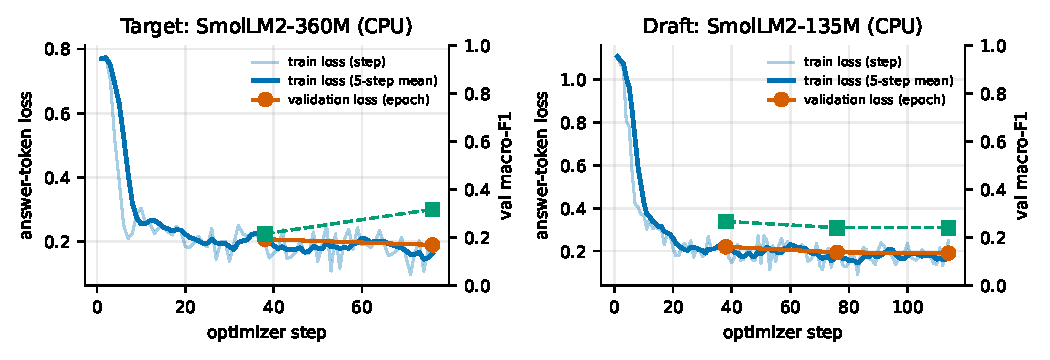
\includegraphics[width=\columnwidth]{fig_training.pdf}
\caption{Config.~B training curves (CPU): target 360M and draft 135M.}\label{fig:trainB}\end{figure}
\begin{table*}[t]\centering\caption{Config.~B (CPU): majority baseline, base zero-shot and fine-tuned SmolLM2-360M on the same rows.}\label{tab:mainB}
\small\begin{tabular}{llrrrrrrr}\toprule
Split & Model & Acc. & mF1 & Incl. acc. & Incl. mF1 & Excl. acc. & Excl. mF1 & Invalid \\\midrule
Val. & majority label & 0.621 & 0.215 & 0.409 & 0.145 & 0.721 & 0.210 & 0 \\
& base zero-shot & 0.495 & 0.229 & 0.136 & 0.113 & 0.664 & 0.276 & 0 \\
& fine-tuned & 0.684 & 0.317 & 0.606 & 0.310 & 0.721 & 0.210 & 0 \\
\midrule
Test & majority label & 0.626 & 0.272 & 0.507 & 0.168 & 0.695 & 0.273 & 0 \\
& base zero-shot & 0.437 & 0.234 & 0.120 & 0.070 & 0.618 & 0.350 & 0 \\
& fine-tuned & 0.626 & 0.333 & 0.507 & 0.247 & 0.695 & 0.273 & 0 \\
\bottomrule\end{tabular}
\end{table*}
\begin{table}[t]\centering\caption{Config.~B fine-tuned model, test split: per-class P, R, F1 and support.}\label{tab:pcBcpu}
\footnotesize\begin{tabular}{llrrrr}\toprule
Scope & Class & P & R & F1 & Support \\\midrule
inclusion & included & 0.444 & 0.296 & 0.356 & 27 \\
 & not included & 0.000 & 0.000 & 0.000 & 7 \\
 & not enough info. & 0.526 & 0.789 & 0.632 & 38 \\
 & not applicable & 0.000 & 0.000 & 0.000 & 3 \\
\midrule
exclusion & excluded & 0.000 & 0.000 & 0.000 & 0 \\
 & not excluded & 0.695 & 1.000 & 0.820 & 91 \\
 & not enough info. & 0.000 & 0.000 & 0.000 & 28 \\
 & not applicable & 0.000 & 0.000 & 0.000 & 12 \\
\bottomrule\end{tabular}
\end{table}
\begin{figure*}[t]\centering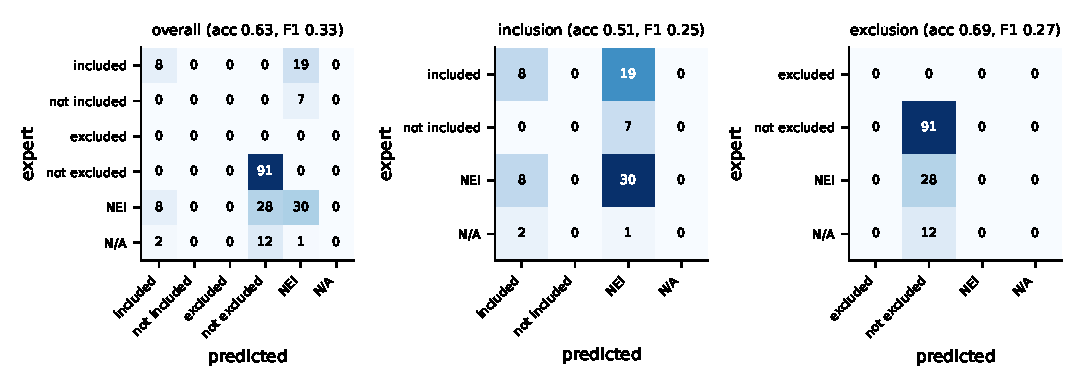
\includegraphics[width=.85\textwidth]{fig_confusion.pdf}
\caption{Config.~B confusion matrices on the test split.}\label{fig:cmB}\end{figure*}
\begin{table}[t]\centering\caption{Config.~B test errors by category.}\label{tab:errcatB}
\small\begin{tabular}{lr}\toprule
Error category & Count \\\midrule
correct & 101 \\
false decision & 50 \\
evidence only & 28 \\
missed decision & 26 \\
na confusion & 1 \\
\bottomrule\end{tabular}
\end{table}

\textbf{Draft model (SmolLM2-135M).} Table~\ref{tab:epochsBd} shows the draft's validation behaviour over three epochs (\DTrainHours{}\,h on the CPU). Validation loss keeps falling (0.220, 0.194, 0.191), but the selection rule (highest validation macro-F1) picks epoch~\DBestEpoch{} (0.267) because macro-F1 is higher there than at epochs 2 and 3 (both 0.241); the differences are a few points on 206 rows and are not meaningful beyond showing that the 135M model learns the answer format and the label prior and little else. This is acceptable for a draft, whose purpose is to propose the target's likely tokens, not to be accurate by itself, but it means that the acceptance rates of the CPU pair were not benchmarked in a stored table (see below) and should not be inferred from the GPU pair.

\textbf{What the laptop is used for.} Configuration~B provides the model of the locally hosted application, whose \emph{Compare decoding} tab measures all four decoding modes live on the user's CPU (Section~\ref{sec:appres}); we did not run the full stored benchmark grid of Section~\ref{sec:kvres}--\ref{sec:specres} on the CPU, because the GPU grid already covers prompt lengths, output lengths, attention shapes and draft settings with a larger, more realistic model and any CPU table would add timings but no new correctness evidence. CPU-specific numbers should therefore be taken from the live tab rather than from this paper.

\begin{table}[t]\centering\caption{Config.~B draft (SmolLM2-135M + LoRA, CPU): validation after each epoch ($^*$ = selected).}\label{tab:epochsBd}
\small\input{generated/tab_epochs_draft.tex}\end{table}



\subsection{Application}
\label{sec:appres}
The application is a self-contained web service: \texttt{python app/server.py} (or \texttt{run\_app.bat}) starts a FastAPI server on \texttt{127.0.0.1:8000}, loads the target and draft models and merges the LoRA adapters in a background thread, and serves a single-page browser interface; no notebook, command-line step or IDE is needed afterwards. The header shows a status indicator (starting, ready, error), the loaded model and adapter, and a persistent banner states that this is an educational screening prototype and not a clinical enrollment decision. Loading takes well under a minute on the laptop; requests that arrive earlier receive a clear ``model not ready'' message instead of an error. If an adapter is missing, the base model is used and the header says so.

\textbf{Screening workflow (Fig.~\ref{fig:app2}).} A user supplies a patient note by pasting text or loading one of the held-out sample patients, and a trial by choosing a sample trial, fetching one from ClinicalTrials.gov by NCT identifier (public metadata only), pasting an ``Inclusion Criteria / Exclusion Criteria'' block that is split into individual criteria, or typing criteria manually. Notes that are not already numbered are split into sentences and numbered from zero, with a preview of the numbering. For every criterion the interface shows the predicted label, the cited sentences quoted from the note, an explanation that only restates the label and the cited text, the raw model output, latency and generated tokens, and, for the sample patients, the dataset's expert label with a match indicator; selecting a criterion highlights its cited sentences in the numbered note (yellow) and the expert's sentences (green marker). The preliminary outcome (here ``Needs more information'') is computed by the explicit rule of Section~III-H and is displayed together with that rule. Missing information is never presented as eligibility: a criterion with no cited sentence is shown with the text ``No supporting sentence cited''.

\textbf{Report export and provenance.} The \emph{Download report} buttons produce a readable HTML report (also suitable for printing to PDF), a Markdown file or a JSON file containing the disclaimer, the trial, the preliminary outcome with its rule, every criterion with label, evidence text and explanation, the numbered note, and provenance: generation time, model, a SHA-256 prefix of the adapter file, the decoding settings and a hash of the note.

\textbf{Input validation and recovery (Fig.~\ref{fig:app3}).} The server validates every request: notes shorter than 20 characters, unknown criterion types, criteria shorter than 3 characters or empty reports are rejected with an explanatory message and HTTP~422; an unreachable registry yields a message asking the user to paste the criteria instead; prompts above 3\,000 tokens are refused rather than silently truncated; and if one criterion fails during a multi-criterion run it is reported as invalid while the others continue. After an error the user corrects the field and runs again without reloading.

\textbf{Inference comparison (Fig.~\ref{fig:app4}).} The \emph{Compare decoding} tab runs the current note and a chosen criterion through the four implemented modes---uncached reference, KV cache, KV cache with tiled attention, and speculative decoding with a selectable draft length---with a warm-up pass and selectable repetitions, optionally forcing a longer output. It reports whether each mode's tokens are identical to the first, prefill, decode and total time, tokens per second, speed-up, memory growth, target forward passes and, for speculative decoding, the acceptance rate, and draws latency and throughput bars. These numbers are measured live on the machine hosting the application, not read from images; the \emph{Experiments} tab additionally renders the stored result files (before/after metrics, KV, attention and speculative benchmarks). In the screenshot, taken while a training job was competing for the same CPU, all four modes return identical tokens, the cache is faster than the reference, our tiled kernel is slower than SDPA inside the decoder, and speculative decoding reaches a 41\% acceptance rate with the un-tuned draft available at that moment.

\begin{figure}[t]\centering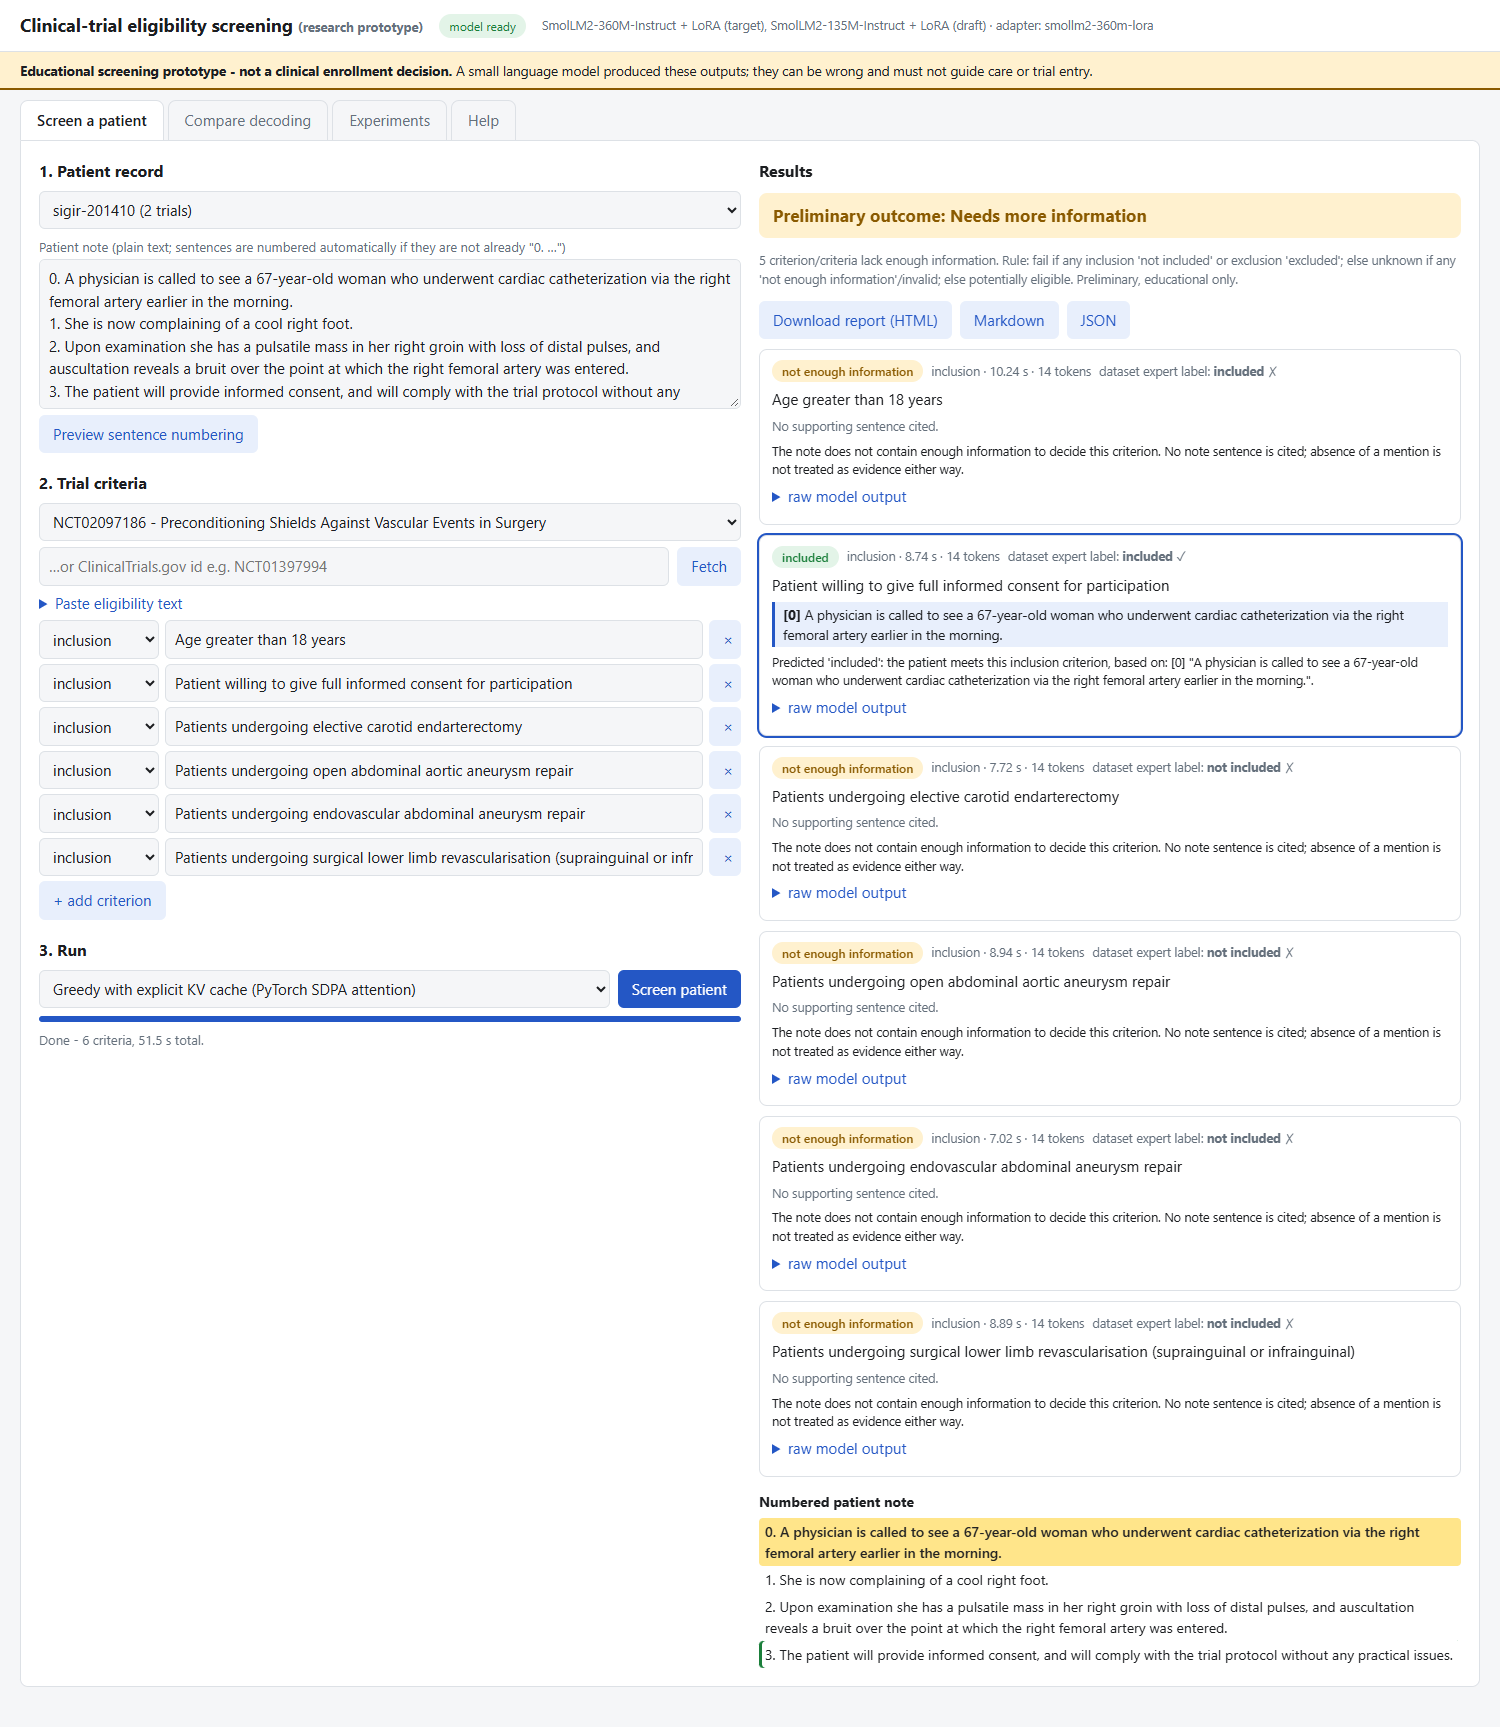
\includegraphics[height=.52\textheight,keepaspectratio]{app_02_results.png}
\caption{Screening workflow: sample patient and trial, six criteria screened, per-criterion label and cited evidence, preliminary outcome, report export buttons, and the numbered note with the selected criterion's evidence highlighted.}\label{fig:app2}\end{figure}
\begin{figure}[t]\centering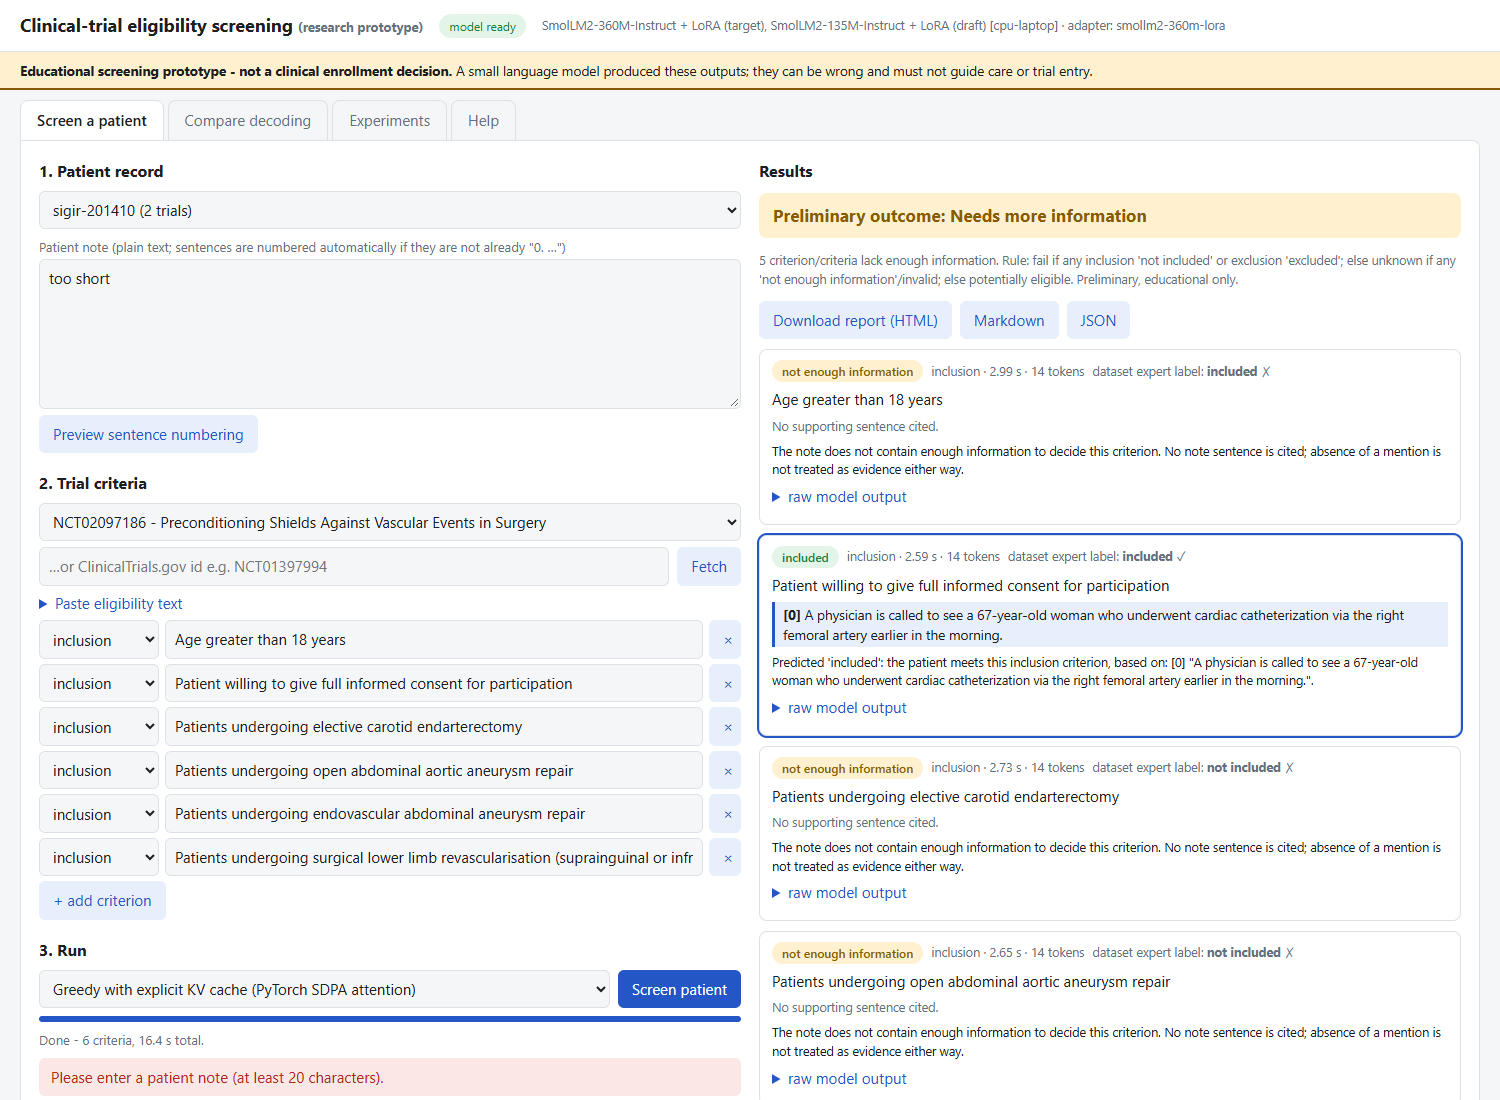
\includegraphics[width=\columnwidth]{app_03_error_recovery.png}
\caption{Recovery from an invalid input: a too-short note is rejected with an explanatory message and the form remains usable.}\label{fig:app3}\end{figure}
\begin{figure}[t]\centering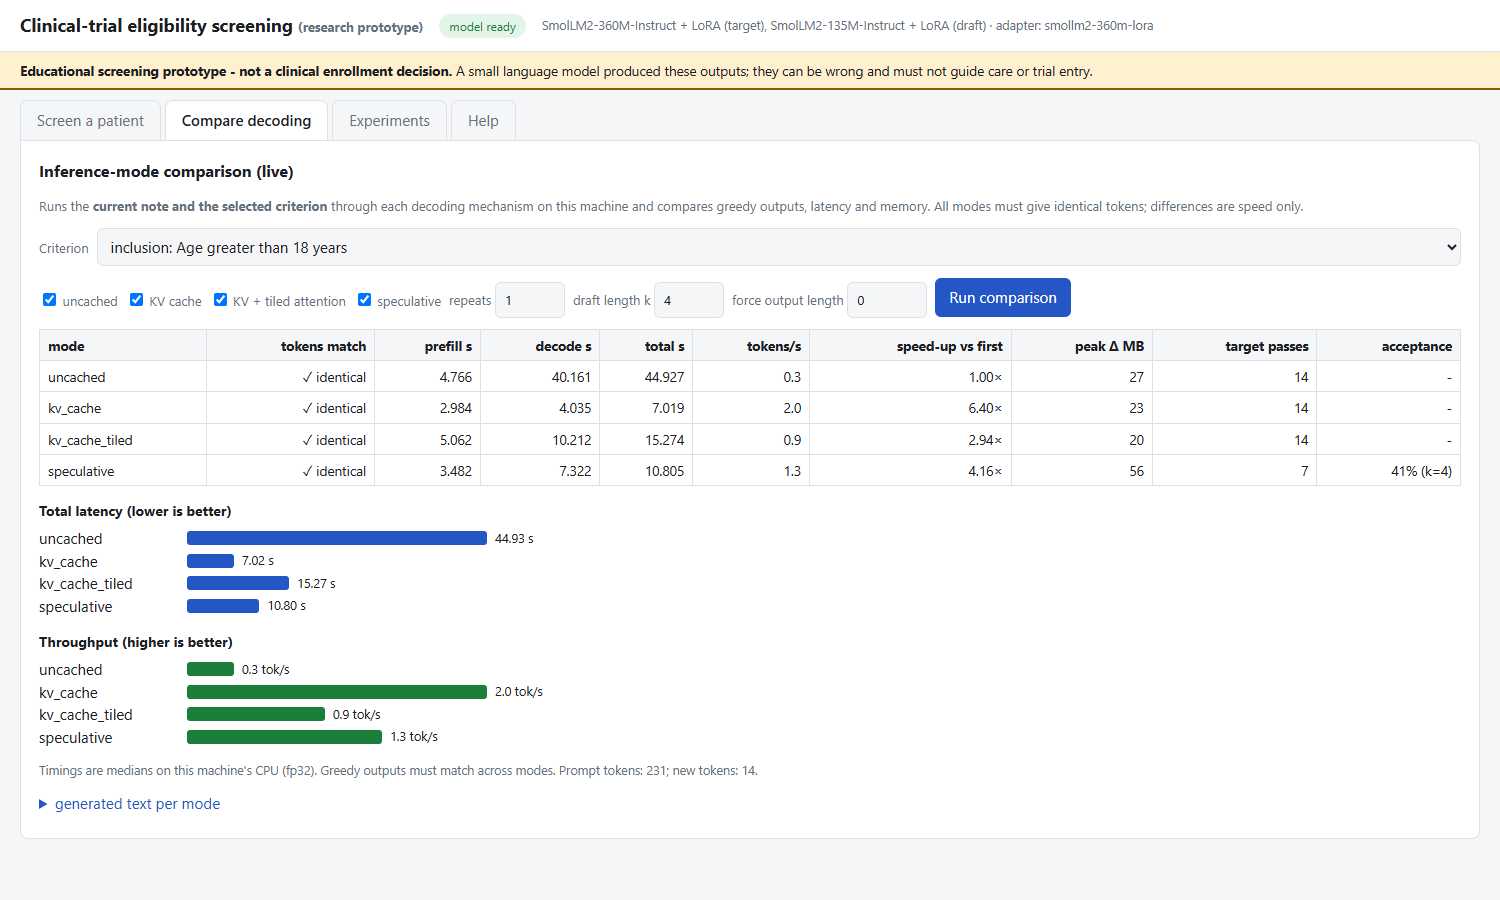
\includegraphics[width=\columnwidth]{app_04_compare.png}
\caption{\emph{Compare decoding} tab: live comparison of the four decoding modes on the same input (timings include contention from a concurrent training job).}\label{fig:app4}\end{figure}


\section{Limitations}
\textbf{Small, clustered test set.} The test split has 8 patients and \NTest{} criteria that are not independent; differences of a few points are within the bootstrap intervals, and rare classes (\emph{not included}, \emph{excluded}) have a handful of examples or none. Conclusions about those classes are therefore weak.

\textbf{Model scale and hardware.} Models of 0.36--1.7B parameters trained for two to four epochs on 602 examples are far from the capability of GPT-4-class systems; we did not tune LoRA rank, learning rate or epoch count beyond the single configuration per model reported, and we did not run multiple seeds, so run-to-run variance is unknown. Epoch selection used validation macro-F1, which moves by several points between epochs and is itself noisy. The GPU numbers come from a shared Kaggle T4 whose clock and neighbours we do not control.

\textbf{Shortness and style of notes.} The corpus contains short synthetic descriptions; real electronic health records are longer, noisier and would need chunking and retrieval before this prompt format applies. The app rejects prompts above 3\,000 tokens rather than truncating silently.

\textbf{Explanations are extractive.} They restate the label and the cited sentences; they are not free-text clinical reasoning and cannot detect an unsupported citation beyond checking that the ID exists in the note.

\textbf{No patient-level ground truth.} The preliminary outcome is a transparent rule over criterion labels; it has not been validated against any patient-trial label and should not be read as one.

\textbf{Benchmark validity.} Timings come from one laptop CPU with background load kept minimal but not zero. Memory is a sampled RSS proxy. The educational tiled attention is pure PyTorch and says nothing about fused GPU kernels; speculative-decoding speed-ups measured here depend on the CPU cost ratio of the two models and on the very short natural outputs.

\textbf{Safety.} The system is an educational screening prototype. It must not be used for enrollment, treatment or any other clinical decision.

\section{Conclusion}
We built, trained and evaluated an end-to-end criterion-level eligibility screener on the TrialGPT annotation corpus with a strictly patient-grouped split, and implemented the Transformer inference mechanisms ourselves rather than through a library switch. Fine-tuning SmolLM2-1.7B with LoRA lifts test macro-F1 from \GBaseMF{} (zero-shot) to \GTestMF{} and accuracy from \GBaseAcc{} to \GTestAcc{}, with evidence F1 \GTestEvF{}; however, the accuracy gain over the \GMajAcc{} majority baseline is not statistically established, the improvement is confined to inclusion criteria, and for exclusion criteria the model almost always answers \emph{not excluded}, treating missing information as a negative finding in 40 of 42 such cases. The explicit KV cache reproduces uncached greedy output exactly and is \GKVSpeedup$\times$ faster at 512+128 tokens at the price of a cache that grows by 393\,kB per token for the 1.7B model; the tiled online-softmax attention matches the reference to $10^{-6}$ and bounds attention memory linearly in sequence length, but is much slower than fused kernels in pure PyTorch; and our greedy speculative decoder is token-exact against the target and against Hugging Face assisted generation, but with a draft that is as deep as the target it is slower than plain decoding on a GPU, which we explain with the cost ratio. Future work should address the exclusion-criterion collapse (class-balanced or cost-sensitive training, an explicit abstention head, or retrieval of relevant sentences), evaluate several seeds, and pair the target with a shallower draft. The system is an educational prototype and not a tool for clinical decisions.


\section*{Acknowledgment and AI-Use Statement}
Claude (Anthropic), used through the Claude Code assistant, supported this work as a coding and writing assistant. It produced first drafts of the source code, scripts and browser application and a first draft of this report, and it helped diagnose and fix errors during development. The author defined the requirements from the assignment brief, provided the inputs and direction for each step, and chose between the alternatives that were considered (for example, moving the main experiments to a free Kaggle GPU, the SmolLM2 model pair, and which experiments to run or to skip). The author ran the GPU fine-tuning, evaluation and benchmarks on Kaggle and resolved the errors that occurred there with the assistant's help; the laptop (CPU) experiments were run locally with the assistant. The author tested the browser application, reviewed the code and the reported results, and reviewed and revised this report. Reused libraries and pre-trained weights (PyTorch, Hugging Face Transformers and PEFT, FastAPI, SmolLM2, Qwen2.5) are cited or named in the text and were tested rather than assumed correct: the re-implemented decoder was checked against the Hugging Face logits, the cache, tiled attention and speculative decoder against reference paths, and all tables are generated by scripts from saved result files. No code or results were taken from the TrialGPT repository; only its public annotation dataset was used. The author is responsible for the submitted work.


\bibliographystyle{IEEEtran}
\bibliography{references}

\end{document}
